\PassOptionsToPackage{unicode=true}{hyperref} % options for packages loaded elsewhere
\PassOptionsToPackage{hyphens}{url}
%
\documentclass[11pt,ignorenonframetext,]{beamer}
\usepackage{pgfpages}
\setbeamertemplate{caption}[numbered]
\setbeamertemplate{caption label separator}{: }
\setbeamercolor{caption name}{fg=normal text.fg}
\beamertemplatenavigationsymbolsempty
% Prevent slide breaks in the middle of a paragraph:
\widowpenalties 1 10000
\raggedbottom
\setbeamertemplate{part page}{
\centering
\begin{beamercolorbox}[sep=16pt,center]{part title}
  \usebeamerfont{part title}\insertpart\par
\end{beamercolorbox}
}
\setbeamertemplate{section page}{
\centering
\begin{beamercolorbox}[sep=12pt,center]{part title}
  \usebeamerfont{section title}\insertsection\par
\end{beamercolorbox}
}
\setbeamertemplate{subsection page}{
\centering
\begin{beamercolorbox}[sep=8pt,center]{part title}
  \usebeamerfont{subsection title}\insertsubsection\par
\end{beamercolorbox}
}
\AtBeginPart{
  \frame{\partpage}
}
\AtBeginSection{
  \ifbibliography
  \else
    \frame{\sectionpage}
  \fi
}
\AtBeginSubsection{
  \frame{\subsectionpage}
}
\usepackage{lmodern}
\usepackage{amssymb,amsmath}
\usepackage{ifxetex,ifluatex}
\usepackage{fixltx2e} % provides \textsubscript
\ifnum 0\ifxetex 1\fi\ifluatex 1\fi=0 % if pdftex
  \usepackage[T1]{fontenc}
  \usepackage[utf8]{inputenc}
  \usepackage{textcomp} % provides euro and other symbols
\else % if luatex or xelatex
  \usepackage{unicode-math}
  \defaultfontfeatures{Ligatures=TeX,Scale=MatchLowercase}
\fi
\usetheme[]{metropolis}
% use upquote if available, for straight quotes in verbatim environments
\IfFileExists{upquote.sty}{\usepackage{upquote}}{}
% use microtype if available
\IfFileExists{microtype.sty}{%
\usepackage[]{microtype}
\UseMicrotypeSet[protrusion]{basicmath} % disable protrusion for tt fonts
}{}
\IfFileExists{parskip.sty}{%
\usepackage{parskip}
}{% else
\setlength{\parindent}{0pt}
\setlength{\parskip}{6pt plus 2pt minus 1pt}
}
\usepackage{hyperref}
\hypersetup{
            pdftitle={Lecture 13},
            pdfborder={0 0 0},
            breaklinks=true}
\urlstyle{same}  % don't use monospace font for urls
\newif\ifbibliography
\usepackage{color}
\usepackage{fancyvrb}
\newcommand{\VerbBar}{|}
\newcommand{\VERB}{\Verb[commandchars=\\\{\}]}
\DefineVerbatimEnvironment{Highlighting}{Verbatim}{commandchars=\\\{\}}
% Add ',fontsize=\small' for more characters per line
\newenvironment{Shaded}{}{}
\newcommand{\AlertTok}[1]{\textcolor[rgb]{1.00,0.00,0.00}{\textbf{#1}}}
\newcommand{\AnnotationTok}[1]{\textcolor[rgb]{0.38,0.63,0.69}{\textbf{\textit{#1}}}}
\newcommand{\AttributeTok}[1]{\textcolor[rgb]{0.49,0.56,0.16}{#1}}
\newcommand{\BaseNTok}[1]{\textcolor[rgb]{0.25,0.63,0.44}{#1}}
\newcommand{\BuiltInTok}[1]{#1}
\newcommand{\CharTok}[1]{\textcolor[rgb]{0.25,0.44,0.63}{#1}}
\newcommand{\CommentTok}[1]{\textcolor[rgb]{0.38,0.63,0.69}{\textit{#1}}}
\newcommand{\CommentVarTok}[1]{\textcolor[rgb]{0.38,0.63,0.69}{\textbf{\textit{#1}}}}
\newcommand{\ConstantTok}[1]{\textcolor[rgb]{0.53,0.00,0.00}{#1}}
\newcommand{\ControlFlowTok}[1]{\textcolor[rgb]{0.00,0.44,0.13}{\textbf{#1}}}
\newcommand{\DataTypeTok}[1]{\textcolor[rgb]{0.56,0.13,0.00}{#1}}
\newcommand{\DecValTok}[1]{\textcolor[rgb]{0.25,0.63,0.44}{#1}}
\newcommand{\DocumentationTok}[1]{\textcolor[rgb]{0.73,0.13,0.13}{\textit{#1}}}
\newcommand{\ErrorTok}[1]{\textcolor[rgb]{1.00,0.00,0.00}{\textbf{#1}}}
\newcommand{\ExtensionTok}[1]{#1}
\newcommand{\FloatTok}[1]{\textcolor[rgb]{0.25,0.63,0.44}{#1}}
\newcommand{\FunctionTok}[1]{\textcolor[rgb]{0.02,0.16,0.49}{#1}}
\newcommand{\ImportTok}[1]{#1}
\newcommand{\InformationTok}[1]{\textcolor[rgb]{0.38,0.63,0.69}{\textbf{\textit{#1}}}}
\newcommand{\KeywordTok}[1]{\textcolor[rgb]{0.00,0.44,0.13}{\textbf{#1}}}
\newcommand{\NormalTok}[1]{#1}
\newcommand{\OperatorTok}[1]{\textcolor[rgb]{0.40,0.40,0.40}{#1}}
\newcommand{\OtherTok}[1]{\textcolor[rgb]{0.00,0.44,0.13}{#1}}
\newcommand{\PreprocessorTok}[1]{\textcolor[rgb]{0.74,0.48,0.00}{#1}}
\newcommand{\RegionMarkerTok}[1]{#1}
\newcommand{\SpecialCharTok}[1]{\textcolor[rgb]{0.25,0.44,0.63}{#1}}
\newcommand{\SpecialStringTok}[1]{\textcolor[rgb]{0.73,0.40,0.53}{#1}}
\newcommand{\StringTok}[1]{\textcolor[rgb]{0.25,0.44,0.63}{#1}}
\newcommand{\VariableTok}[1]{\textcolor[rgb]{0.10,0.09,0.49}{#1}}
\newcommand{\VerbatimStringTok}[1]{\textcolor[rgb]{0.25,0.44,0.63}{#1}}
\newcommand{\WarningTok}[1]{\textcolor[rgb]{0.38,0.63,0.69}{\textbf{\textit{#1}}}}
\usepackage{longtable,booktabs}
\usepackage{caption}
% These lines are needed to make table captions work with longtable:
\makeatletter
\def\fnum@table{\tablename~\thetable}
\makeatother
\setlength{\emergencystretch}{3em}  % prevent overfull lines
\providecommand{\tightlist}{%
  \setlength{\itemsep}{0pt}\setlength{\parskip}{0pt}}
\setcounter{secnumdepth}{0}

% set default figure placement to htbp
\makeatletter
\def\fps@figure{htbp}
\makeatother

\usepackage{geometry}
\usepackage{graphicx}

\usepackage{bbold}
\usepackage{lmodern}


\usepackage{url}		% produces hyperlinks

\usepackage{colortbl}	% allows for color usage in tables
\usepackage{multirow}	% allows for rows that span multiple rows in tables

\usepackage{color}          	% gives color options
\usepackage{xcolor}		% this package has a variety of color options

\usepackage{multicol}
\usepackage{textcomp}

\usepackage{setspace}
\usepackage{changepage}
\usepackage{isotope}

\singlespacing

\def\begincol{\begin{column}}
\def\endcol{\end{column}}

\def\begincols{\begin{columns}}
\def\endcols{\end{columns}}

%%%%%%%%%%%%%%%%
% Small code output
%%%%%%%%%%%%%%%%

%% change fontsize of R code

\makeatletter
\@ifundefined{Shaded}{\newenvironment{Shaded}{}{}}{}
\makeatother


\let\oldShaded\Shaded
\let\endoldShaded\endShaded
\renewenvironment{Shaded}{\footnotesize\begin{spacing}{0.9}\oldShaded}{\endoldShaded\end{spacing}}

%% change fontsize of output
\let\oldverbatim\verbatim
\let\endoldverbatim\endverbatim
\renewenvironment{verbatim}{\footnotesize\begin{spacing}{0.9}\oldverbatim}{\endoldverbatim\end{spacing}}


\newcommand{\tinyoutput}{
  \renewenvironment{Shaded}{\tiny\begin{spacing}{0.9}\oldShaded}{\endoldShaded\end{spacing}}
  \renewenvironment{verbatim}{\tiny\begin{spacing}{0.9}\oldverbatim}{\endoldverbatim\end{spacing}}
}

\newcommand{\scriptoutput}{
  \renewenvironment{Shaded}{\scriptsize\begin{spacing}{0.9}\oldShaded}{\endoldShaded\end{spacing}}
  \renewenvironment{verbatim}{\scriptsize\begin{spacing}{0.9}\oldverbatim}{\endoldverbatim\end{spacing}}
}

\newcommand{\footnoteoutput}{
  \renewenvironment{Shaded}{\footnotesize\begin{spacing}{0.9}\oldShaded}{\endoldShaded\end{spacing}}
  \renewenvironment{verbatim}{\footnotesize\begin{spacing}{0.9}\oldverbatim}{\endoldverbatim\end{spacing}}
}

%\newcommand{\verbatimfont}[1]{\renewcommand{\verbatim@font}{\ttfamily#1}}


%%%%%%%%%%%%%%%%
% Custom Colors
%%%%%%%%%%%%%%%%

\definecolor{redhl}{rgb}{0.98,0.29,0.28}
\definecolor{yellowhl}{rgb}{0.98,0.87,0.28}


\xdefinecolor{oiBlue}{rgb}{0.15, 0.35, 0.55}
\xdefinecolor{gray}{rgb}{0.5, 0.5, 0.5}
\xdefinecolor{darkGray}{rgb}{0.3, 0.3, 0.3}
\xdefinecolor{darkerGray}{rgb}{0.2, 0.2, 0.2}
\xdefinecolor{rubineRed}{rgb}{0.89,0,0.30}
\xdefinecolor{linkCol}{rgb}{0.11,0.49,0.95}	
\xdefinecolor{irishGreen}{rgb}{0,0.60,0}	
\xdefinecolor{darkturquoise}{rgb}{0.44, 0.58, 0.86}
\definecolor{lightGreen}{rgb}{0.533,0.765,0.42}
%\xdefinecolor{hlblue}{rgb}{0.051,0.65,1}
\xdefinecolor{hlblue}{rgb}{ 0.055, 0.639, 0.831}
\definecolor{light}{rgb}{.337,.608,.741}
\definecolor{dark}{rgb}{.337,.608,.741}

\definecolor{cpink}{rgb}{0.93, 0.23, 0.51}

%%%%%%%%%%%%%%%%
% Custom Commands
%%%%%%%%%%%%%%%%

% text colors
\newcommand{\red}[1]{\textit{\textcolor{rubineRed}{#1}}}
\newcommand{\orange}[1]{\textit{\textcolor{orange}{#1}}}
\newcommand{\pink}[1]{\textit{\textcolor{rubineRed!90!white!50}{#1}}}
\newcommand{\green}[1]{\textit{\textcolor{irishGreen}{#1}}}
\newcommand{\blue}[1]{\textit{\textcolor{darkturquoise}{#1}}}
\newcommand{\light}[1]{\textcolor{light}{\textbf{#1}}}
\newcommand{\dark}[1]{\textcolor{dark}{#1}}
\newcommand{\gray}[1]{\textcolor{gray}{#1}}


% mail
\newcommand{\mail}[1]{\href{mailto:#1}{\textit{\textcolor{linkCol}{#1}}}}

% highlighting: hl, hlGr, mathhl
\newcommand{\hl}[1]{\textit{\textcolor{hlblue}{#1}}}
\newcommand{\hlGr}[1]{\textit{\textcolor{lightGreen}{#1}}}
\newcommand{\hlRd}[1]{\textit{\textcolor{rubineRed}{#1}}}
\newcommand{\mathhl}[1]{\textcolor{hlblue}{\ensuremath{#1}}}
\newcommand{\hlr}[1]{\fcolorbox{redhl}{white}{$\displaystyle #1$}}
\newcommand{\hly}[1]{\fcolorbox{yellowhl}{white}{$\displaystyle #1$}}


\newcommand{\vvfill}{\vskip0pt plus 1filll}

\DeclareMathOperator*{\argmin}{arg\,min}
\DeclareMathOperator*{\argmax}{arg\,max}

\title{Lecture 13}
\providecommand{\subtitle}[1]{}
\subtitle{Gaussian Process Models - Part 2}
\date{10/19/2018}

\begin{document}
\frame{\titlepage}

\hypertarget{eda-and-gps}{%
\section{EDA and GPs}\label{eda-and-gps}}

\begin{frame}[t]{Variogram}
\protect\hypertarget{variogram}{}

When fitting a Gaussian process model, it is often difficult to fit the
covariance parameters (hard to identify). Today we will discuss some EDA
approaches for getting a sense of the values for the scale, range and
nugget parameters.

\pause

From the spatial modeling literature the typical approach is to examine
an \emph{empirical variogram}, first we will define the
\emph{theoretical variogram} and its connection to the covariance.

\vspace{2mm}

\pause

Variogram: \[
2 \gamma(t_i, t_j) = Var(Y(t_i) - Y(t_j))
\] where \(\gamma(t_i, t_j)\) is known as the semivariogram.

\end{frame}

\begin{frame}[t]{Some Properties of the theoretical Variogram /
Semivariogram}
\protect\hypertarget{some-properties-of-the-theoretical-variogram-semivariogram}{}

\vspace{-2mm}

\begin{itemize}
\tightlist
\item
  are non-negative \footnotesize \[\gamma(t_i, t_j) \geq 0\] \normalsize
\end{itemize}

\pause

\vspace{2mm}

\begin{itemize}
\tightlist
\item
  are equal to 0 at distance 0 \footnotesize \[\gamma(t_i, t_i) = 0\]
  \normalsize
\end{itemize}

\pause

\vspace{2mm}

\begin{itemize}
\tightlist
\item
  are symmetric \footnotesize \[\gamma(t_i, t_j) = \gamma(t_j, t_i)\]
  \normalsize
\end{itemize}

\pause

\vspace{2mm}

\begin{itemize}
\tightlist
\item
  if observations are independent
  \footnotesize \[2\gamma(t_i, t_j) = Var(Y(t_i)) + Var(Y(t_j)) \quad \text{ for all } i \ne j\]
  \normalsize
\end{itemize}

\pause

\vspace{2mm}

\begin{itemize}
\tightlist
\item
  if the process \emph{is not} stationary \footnotesize
  \[2\gamma(t_i, t_j) = Var\big(Y(t_i)\big) + Var\big(Y(t_j)\big) - 2 \, Cov\big(Y(t_i),Y(t_j)\big)\]
\end{itemize}

\pause

\vspace{2mm}

\begin{itemize}
\tightlist
\item
  if the process \emph{is} stationary \footnotesize \[\begin{aligned}
  2\gamma(t_i, t_j) 
  &= 2Var\big(Y(t_i)\big) - 2 \, Cov\big(Y(t_i),Y(t_j)\big)
  \end{aligned}\]
\end{itemize}

\end{frame}

\begin{frame}[t]{Empirical Semivariogram}
\protect\hypertarget{empirical-semivariogram}{}

We will assume that our process of interest is stationary, in which case
we will parameterize the semivariagram in terms of \(h = |t_i - t_j|\).

\vspace{3mm}

Empirical Semivariogram:
\[ \hat{\gamma}(h) = \frac{1}{2 \, N(h)} \sum_{|t_i-t_j| \in (h-\epsilon,h+\epsilon)} (Y(t_i) - Y(t_j))^2 \]

\pause

Practically, for any data set with \(n\) observations there are
\({n \choose 2} + n\) possible data pairs to examine. Each individually
is not very informative, so we aggregate into bins and calculate the
empirical semivariogram for each bin.

\end{frame}

\begin{frame}{Connection to Covariance}
\protect\hypertarget{connection-to-covariance}{}

\end{frame}

\begin{frame}{Covariance vs Semivariogram - Exponential}
\protect\hypertarget{covariance-vs-semivariogram---exponential}{}

\begin{center}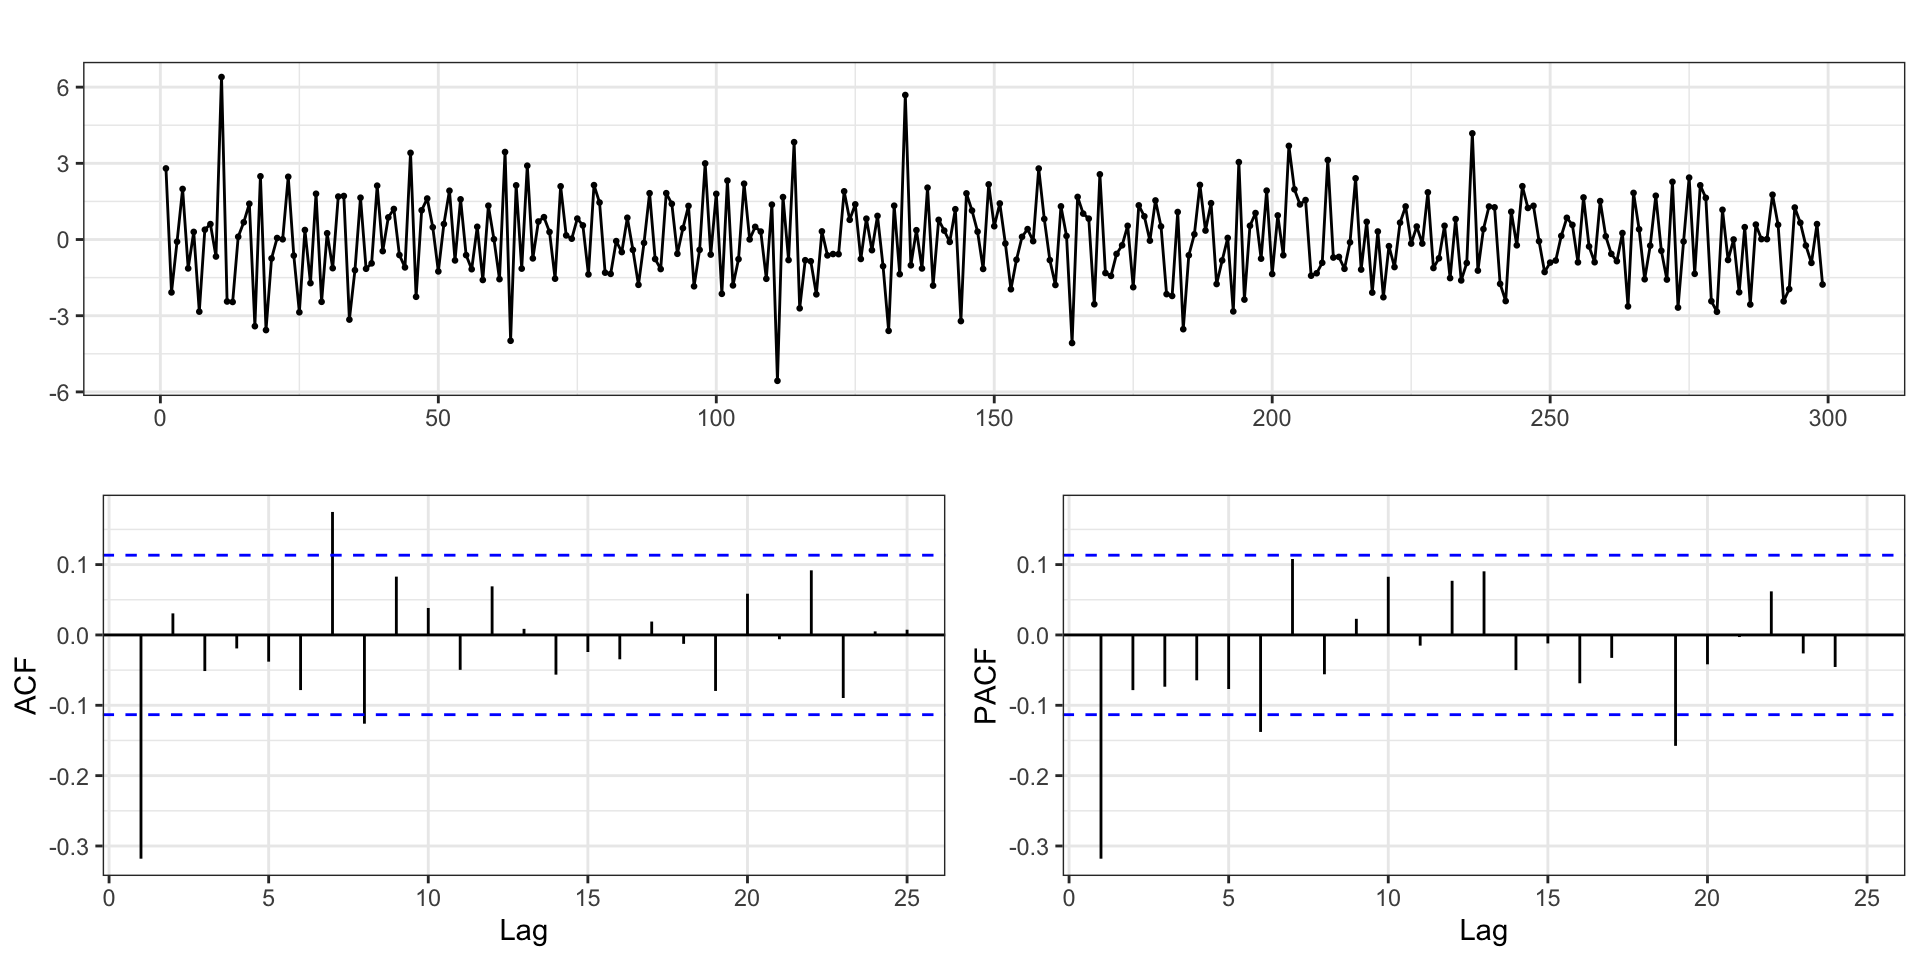
\includegraphics[width=\textwidth]{Lec13_files/figure-beamer/unnamed-chunk-2-1} \end{center}

\end{frame}

\begin{frame}{Covariance vs Semivariogram - Square Exponential}
\protect\hypertarget{covariance-vs-semivariogram---square-exponential}{}

\begin{center}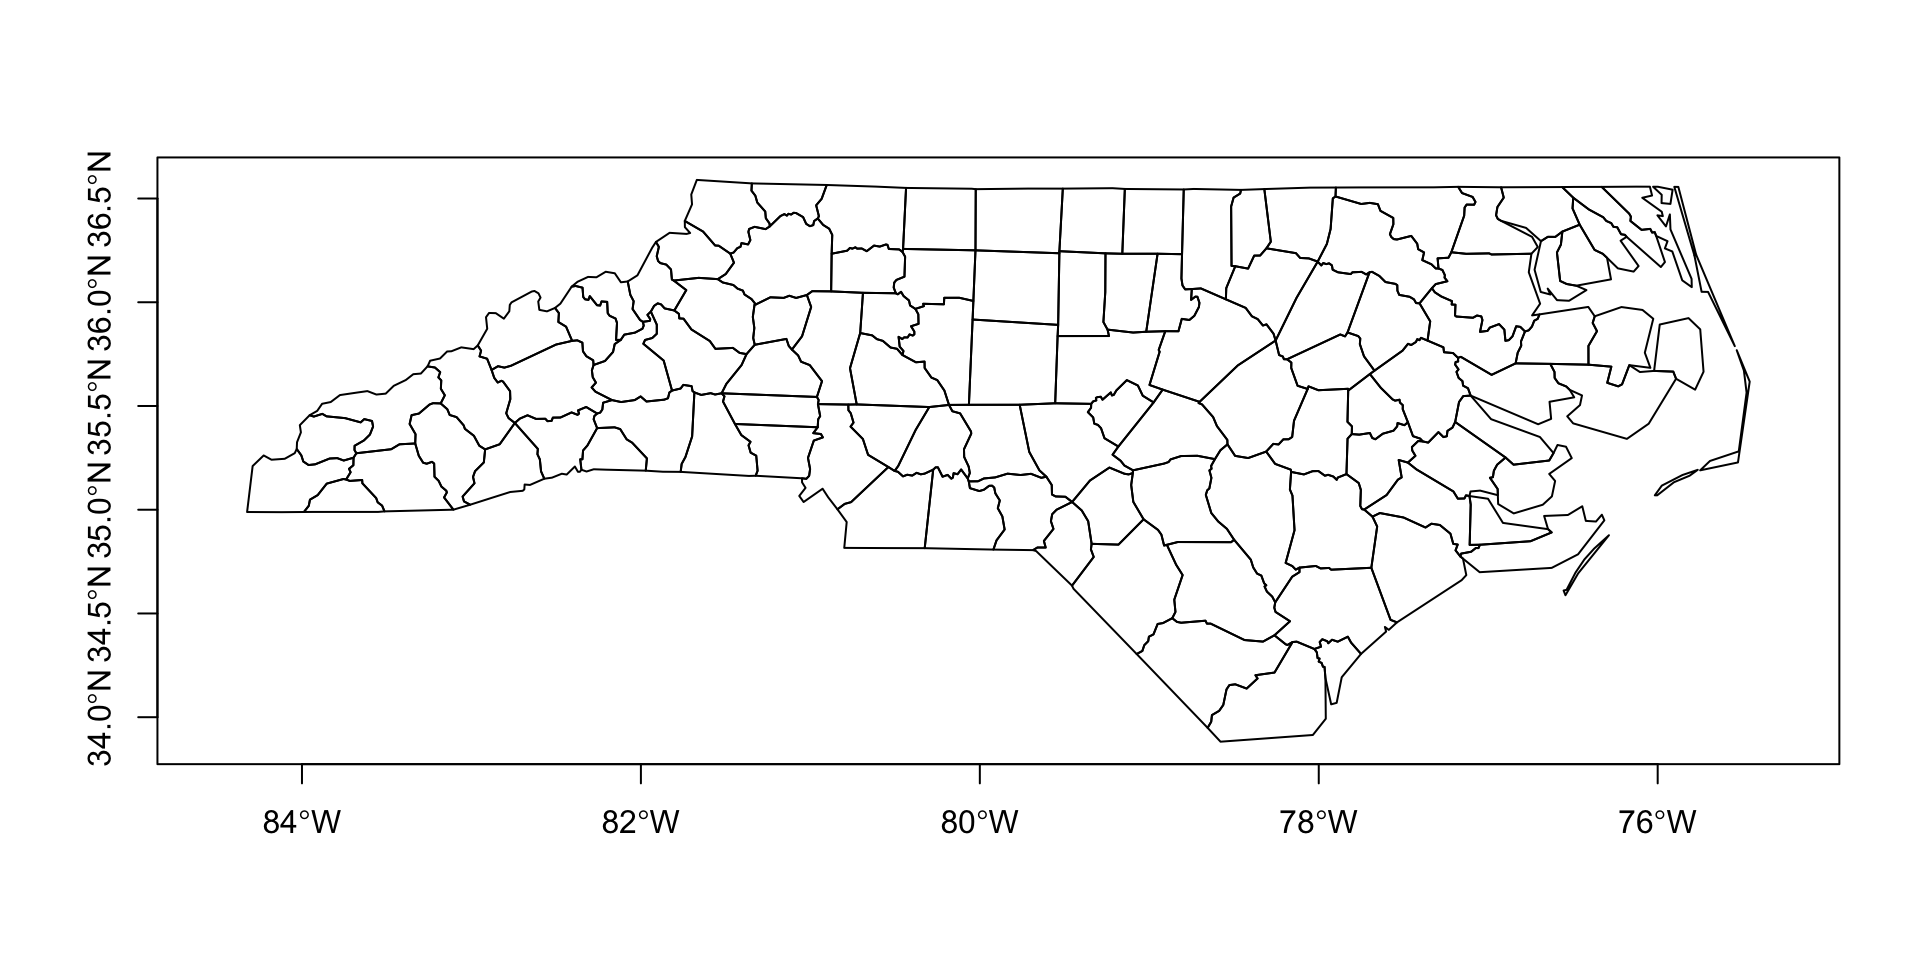
\includegraphics[width=\textwidth]{Lec13_files/figure-beamer/unnamed-chunk-3-1} \end{center}

\end{frame}

\begin{frame}{From last time}
\protect\hypertarget{from-last-time}{}

\begin{center}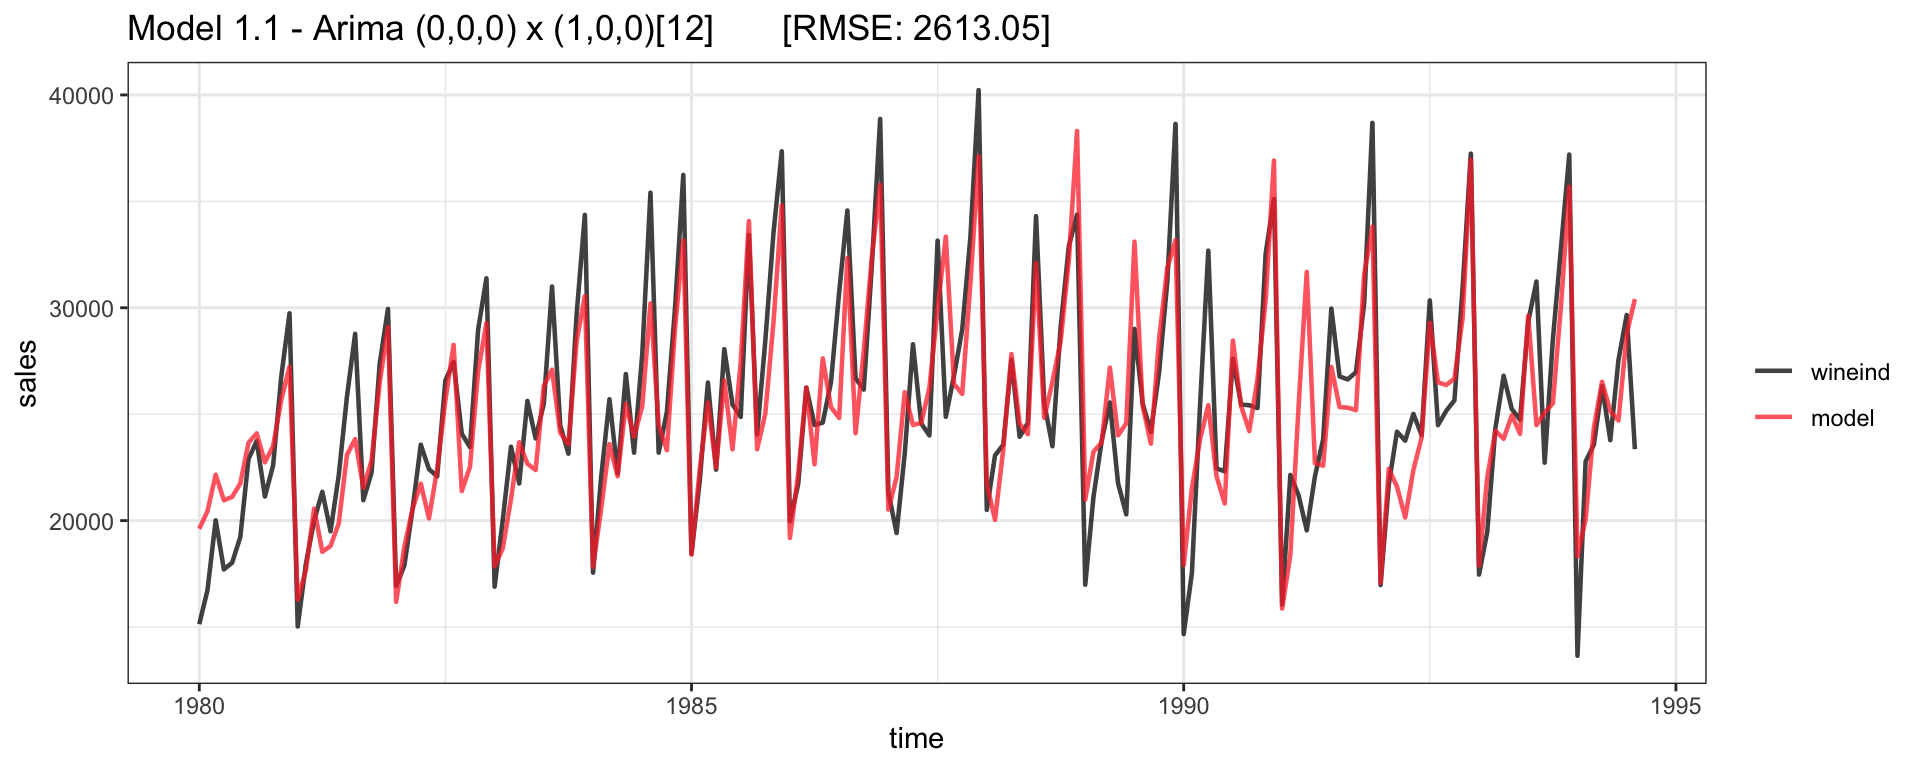
\includegraphics[width=\textwidth]{Lec13_files/figure-beamer/unnamed-chunk-4-1} \end{center}

\end{frame}

\begin{frame}{Empirical semivariogram - no bins / cloud}
\protect\hypertarget{empirical-semivariogram---no-bins-cloud}{}

\begin{center}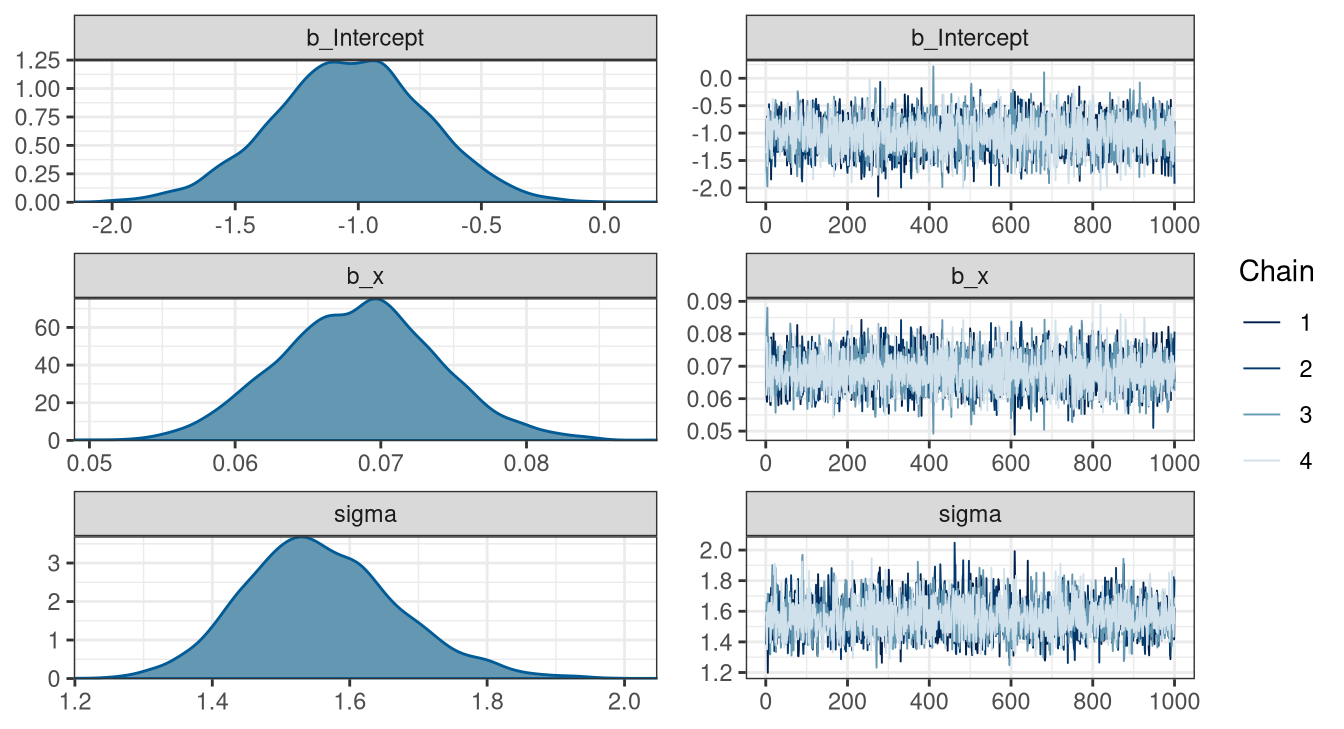
\includegraphics[width=\textwidth]{Lec13_files/figure-beamer/unnamed-chunk-5-1} \end{center}

\end{frame}

\begin{frame}{Empirical semivariogram (binned)}
\protect\hypertarget{empirical-semivariogram-binned}{}

\begin{center}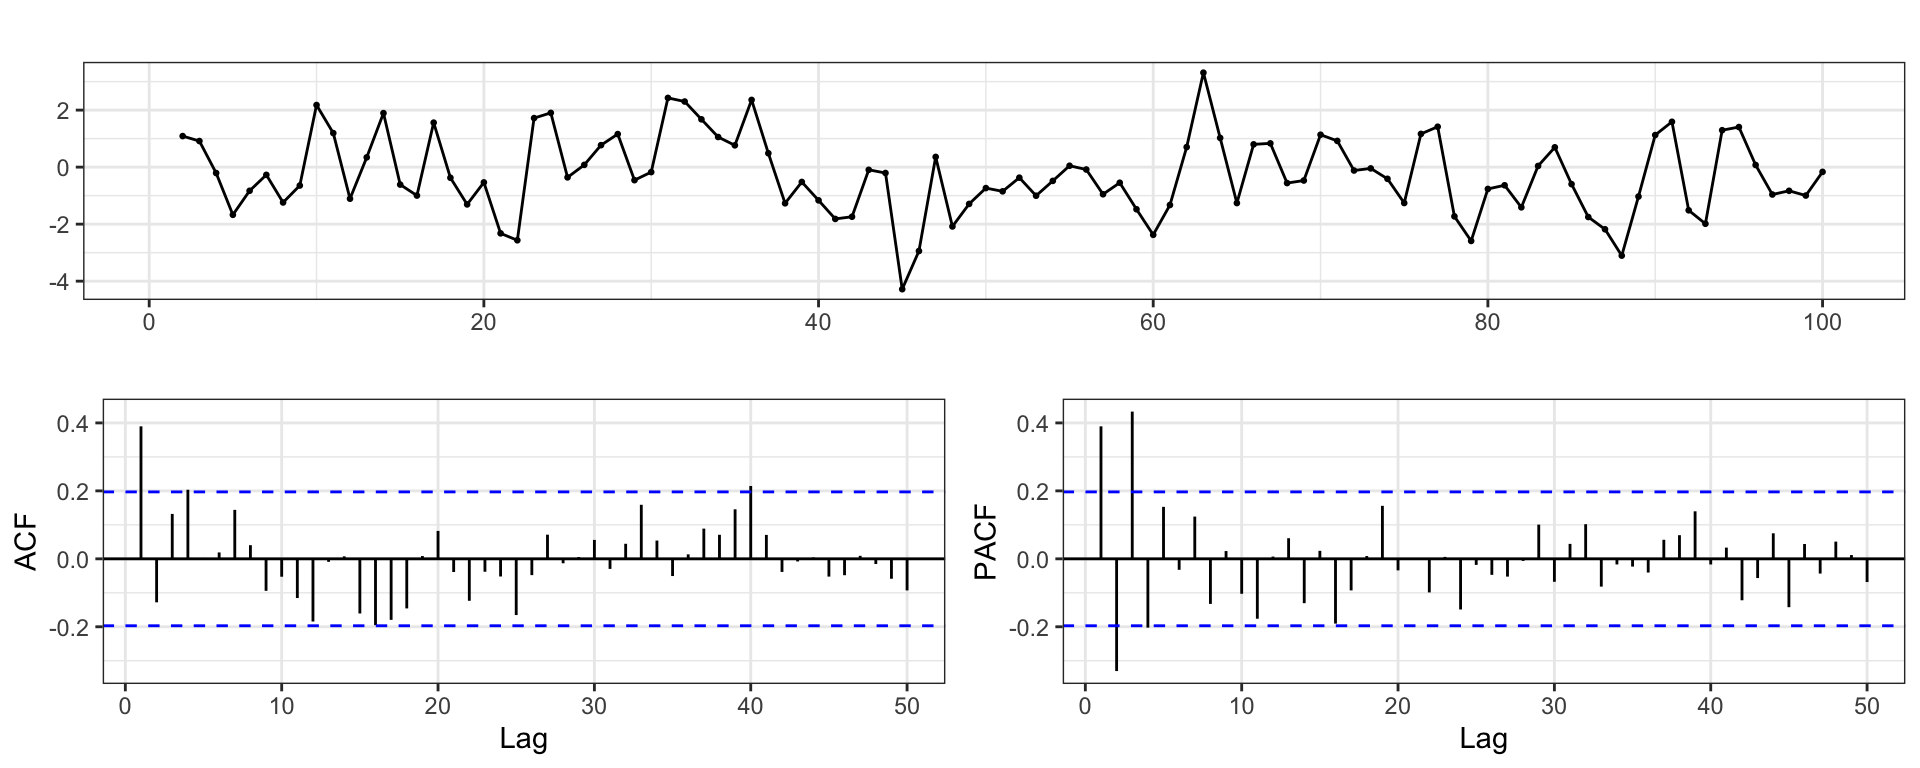
\includegraphics[width=\textwidth]{Lec13_files/figure-beamer/unnamed-chunk-6-1} \end{center}

\end{frame}

\begin{frame}{Empirical semivariogram (binned + n)}
\protect\hypertarget{empirical-semivariogram-binned-n}{}

\begin{center}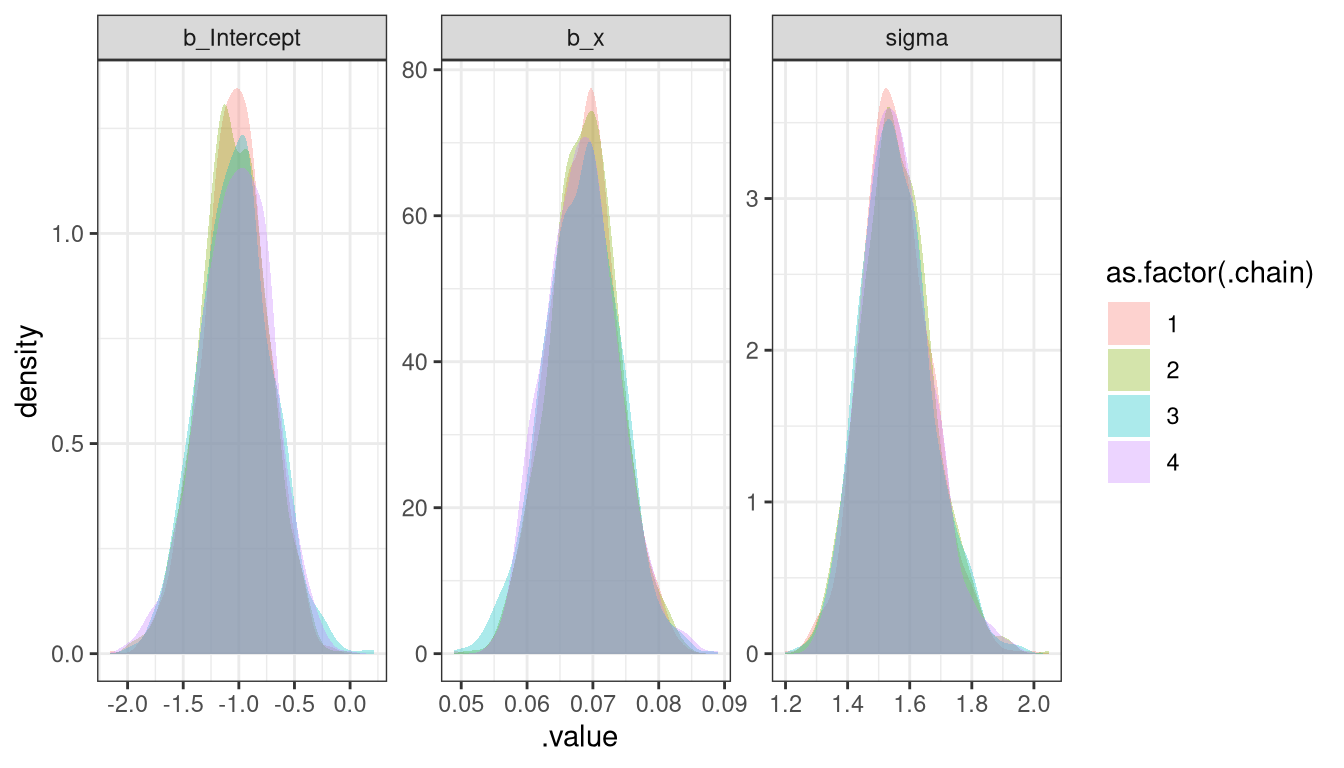
\includegraphics[width=\textwidth]{Lec13_files/figure-beamer/unnamed-chunk-7-1} \end{center}

\end{frame}

\begin{frame}{Theoretical vs empirical semivariogram}
\protect\hypertarget{theoretical-vs-empirical-semivariogram}{}

After fitting the model last time we came up with a posterior median of
\(\sigma^2 = 1.73\), \(l=7.01\), and \$\sigma\^{}2\_w = 0.13 for a
square exponential covariance.

\pause

\scriptsize

\[ 
\begin{aligned}
Cov(h) &= \sigma^2 \exp\big(-(h\,l)^2\big) + \sigma^2_w \symbf{1}_{h=0}\\
\gamma(h) 
  &= \sigma^2 + \sigma^2_w - \sigma^2 \exp\big(-(h\,l)^2\big) \\
  &= 1.73 + 0.13 - 1.73 \exp\big(-(7.01\, h)^2\big)
\end{aligned}
\]

\pause

\begin{center}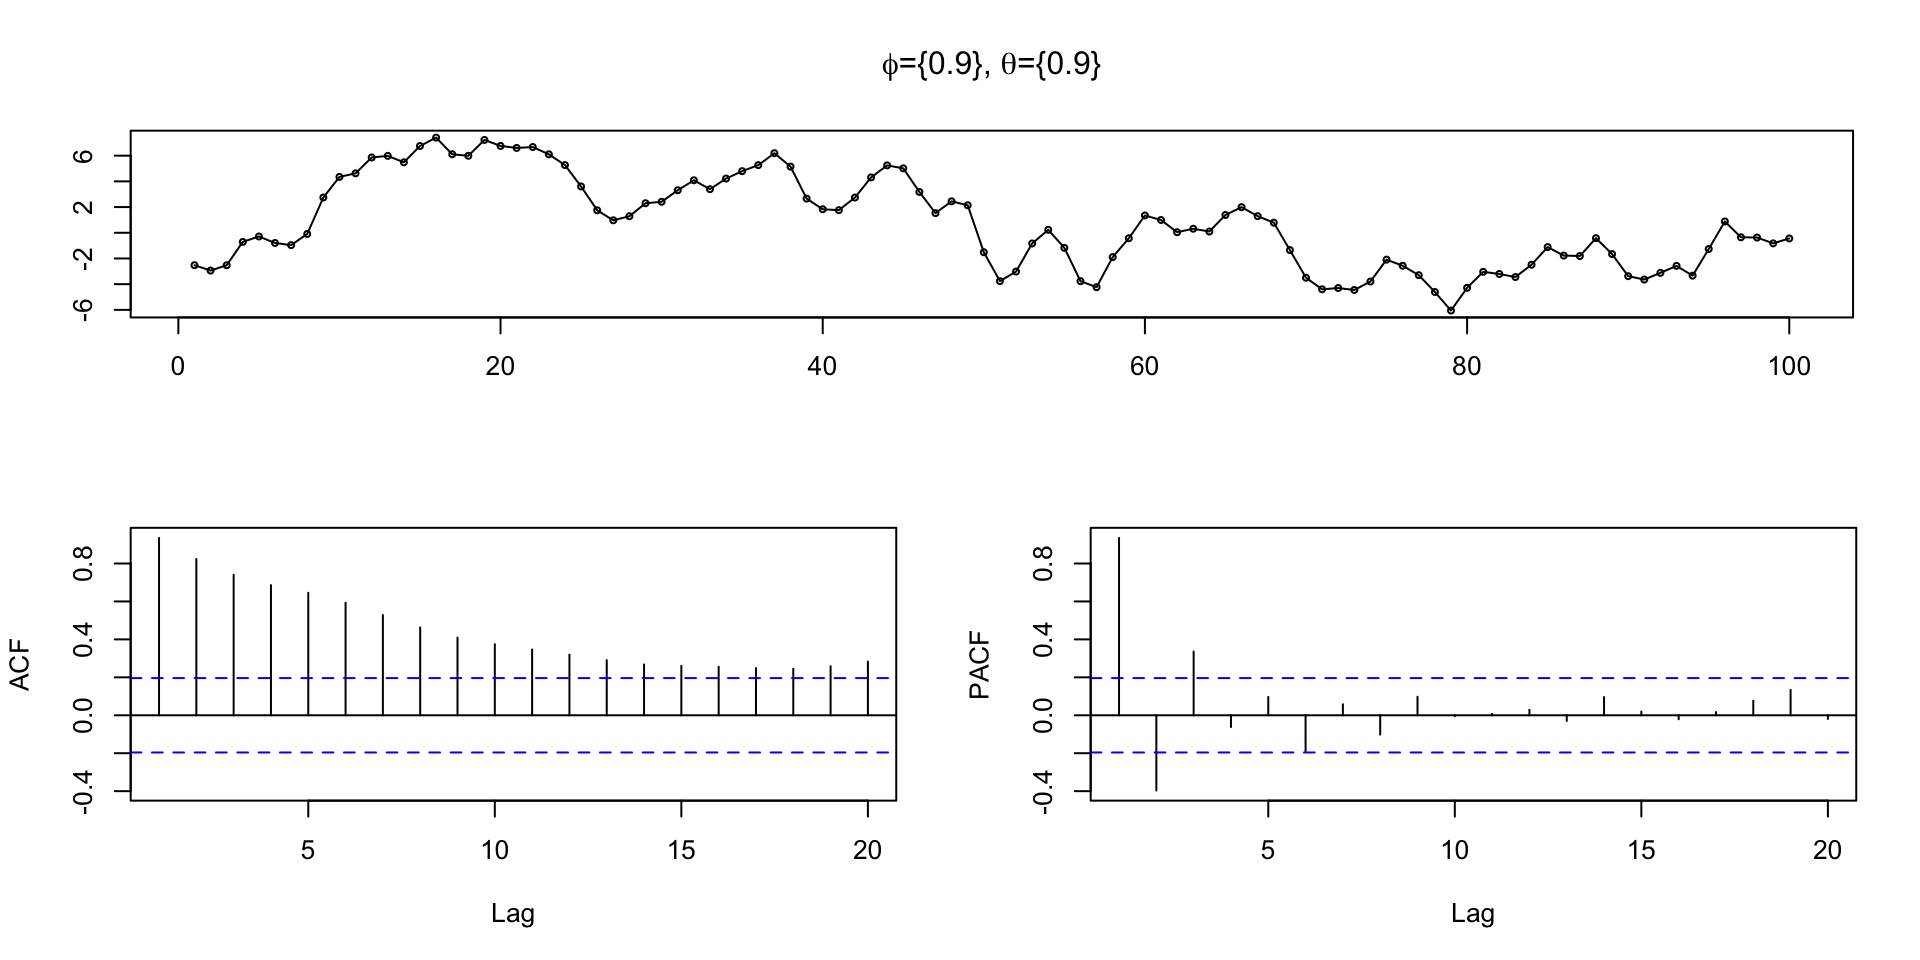
\includegraphics[width=\textwidth]{Lec13_files/figure-beamer/unnamed-chunk-9-1} \end{center}

\end{frame}

\begin{frame}{Variogram features}
\protect\hypertarget{variogram-features}{}

\begin{center}
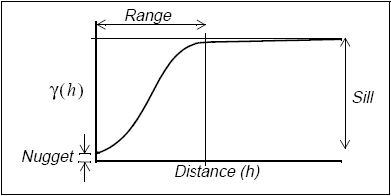
\includegraphics[width=0.7\textwidth]{figs/variogram.png}
\end{center}

\end{frame}

\hypertarget{pm2.5-example}{%
\section{PM2.5 Example}\label{pm2.5-example}}

\begin{frame}{FRN Data}
\protect\hypertarget{frn-data}{}

Measured PM2.5 data from an EPA monitoring station in Columbia, NJ.

\begin{center}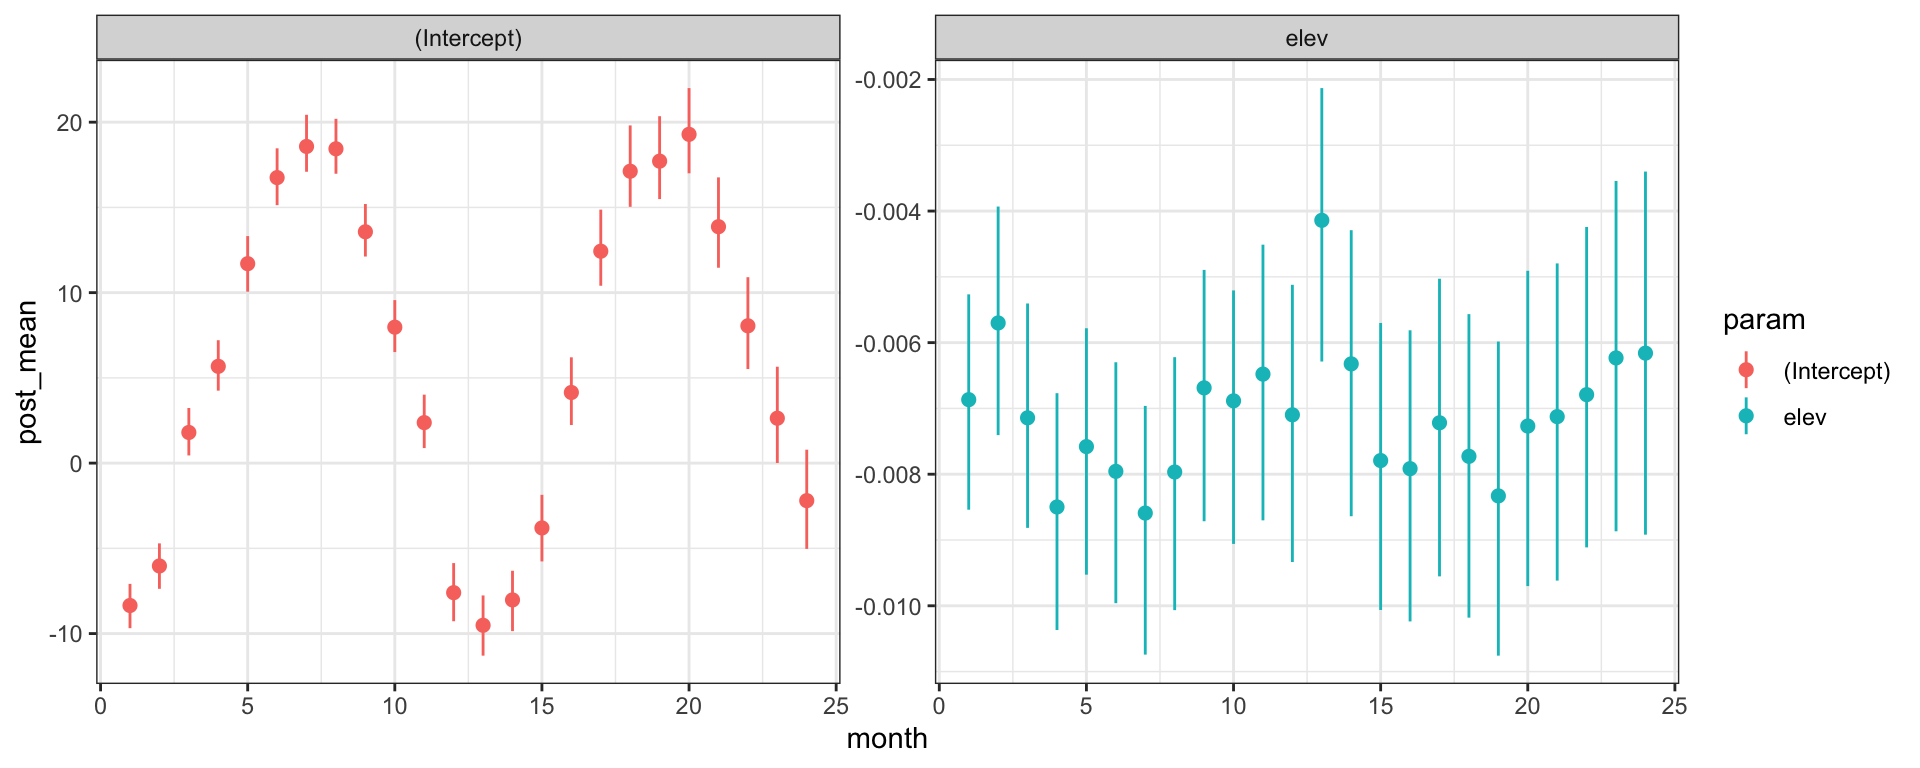
\includegraphics[width=\textwidth]{Lec13_files/figure-beamer/unnamed-chunk-10-1} \end{center}

\end{frame}

\begin{frame}{FRN Data}
\protect\hypertarget{frn-data-1}{}

\footnotesize

\begin{longtable}[]{@{}lrrrlr@{}}
\toprule
site & latitude & longitude & pm25 & date & day\tabularnewline
\midrule
\endhead
230031011 & 46.682 & -68.016 & 8.9 & 2007-01-03 & 3\tabularnewline
230031011 & 46.682 & -68.016 & 10.4 & 2007-01-06 & 6\tabularnewline
230031011 & 46.682 & -68.016 & 9.7 & 2007-01-15 & 15\tabularnewline
230031011 & 46.682 & -68.016 & 7.5 & 2007-01-18 & 18\tabularnewline
230031011 & 46.682 & -68.016 & 4.6 & 2007-01-21 & 21\tabularnewline
230031011 & 46.682 & -68.016 & 9.5 & 2007-01-24 & 24\tabularnewline
230031011 & 46.682 & -68.016 & 9.0 & 2007-01-27 & 27\tabularnewline
230031011 & 46.682 & -68.016 & 16.2 & 2007-01-30 & 30\tabularnewline
230031011 & 46.682 & -68.016 & 9.1 & 2007-02-05 & 36\tabularnewline
230031011 & 46.682 & -68.016 & 19.9 & 2007-02-11 & 42\tabularnewline
230031011 & 46.682 & -68.016 & 11.5 & 2007-02-14 & 45\tabularnewline
230031011 & 46.682 & -68.016 & 6.5 & 2007-02-17 & 48\tabularnewline
230031011 & 46.682 & -68.016 & 14.7 & 2007-02-23 & 54\tabularnewline
230031011 & 46.682 & -68.016 & 14.1 & 2007-02-26 & 57\tabularnewline
230031011 & 46.682 & -68.016 & 13.3 & 2007-03-01 & 60\tabularnewline
230031011 & 46.682 & -68.016 & 8.6 & 2007-03-04 & 63\tabularnewline
230031011 & 46.682 & -68.016 & 9.0 & 2007-03-07 & 66\tabularnewline
230031011 & 46.682 & -68.016 & 14.0 & 2007-03-10 & 69\tabularnewline
230031011 & 46.682 & -68.016 & 8.6 & 2007-03-13 & 72\tabularnewline
230031011 & 46.682 & -68.016 & 10.3 & 2007-03-16 & 75\tabularnewline
\bottomrule
\end{longtable}

\end{frame}

\begin{frame}{Empirical Variogram}
\protect\hypertarget{empirical-variogram}{}

\begin{center}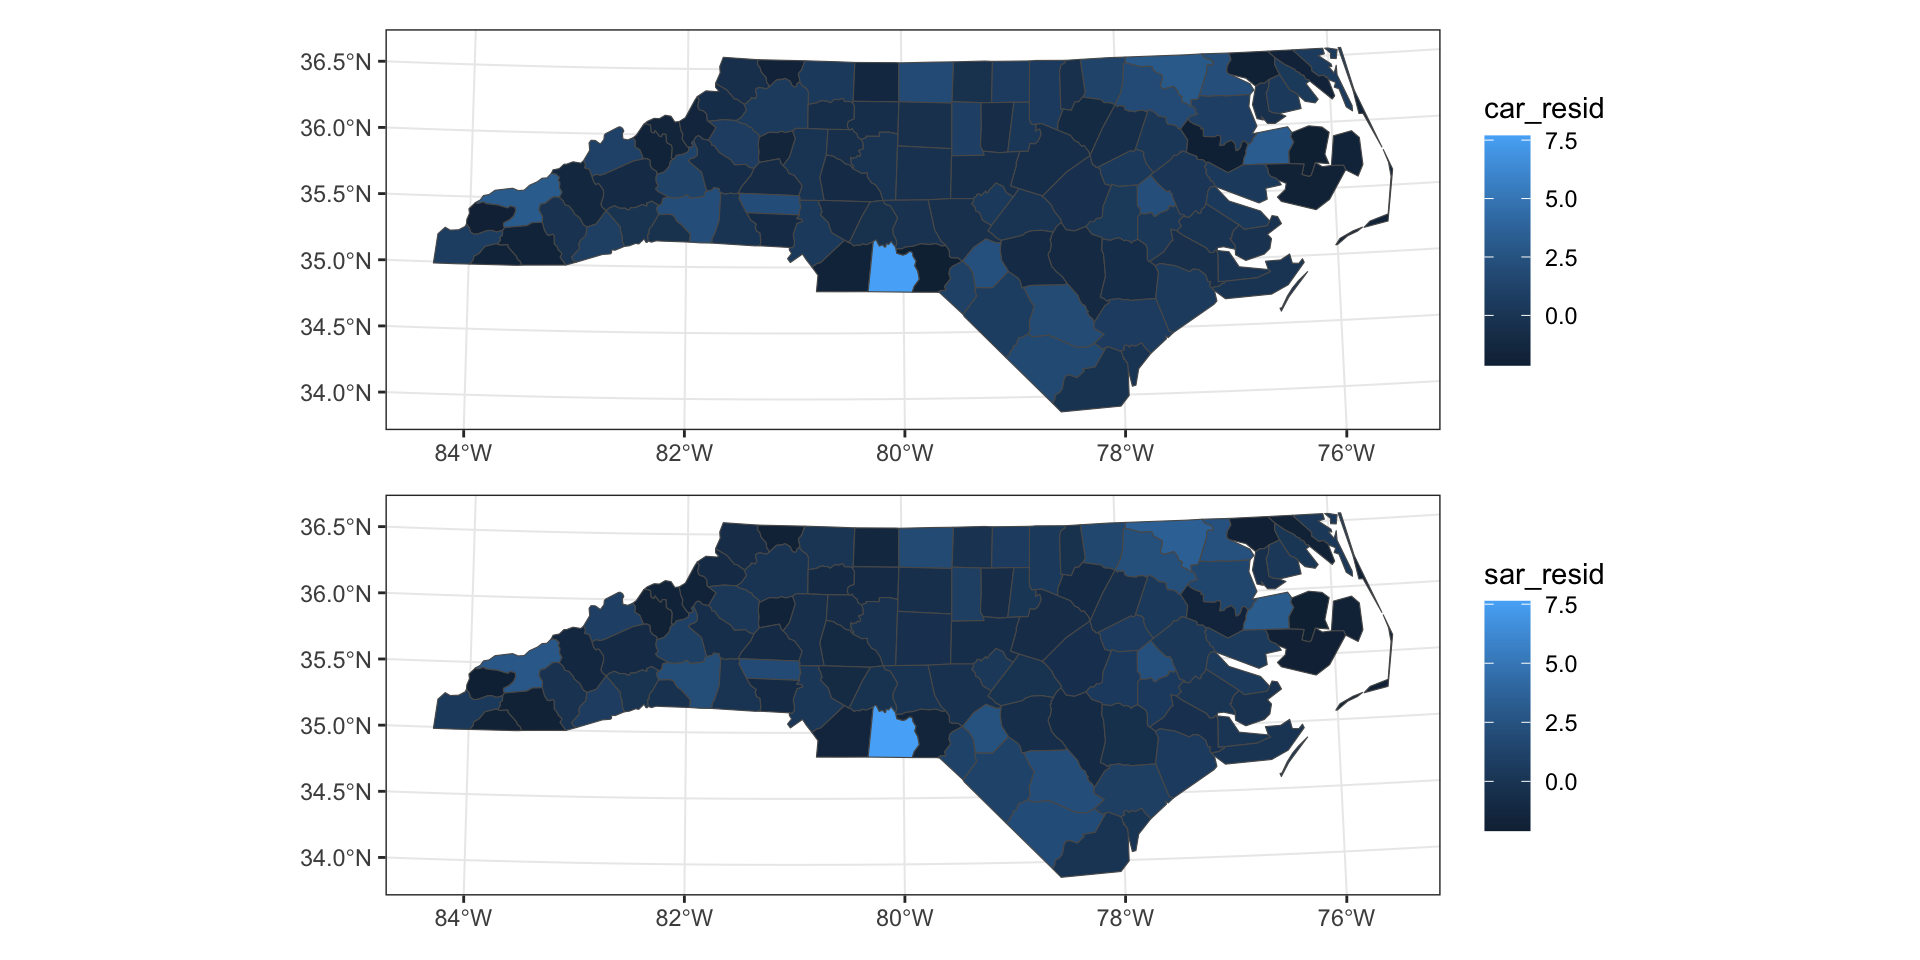
\includegraphics[width=\textwidth]{Lec13_files/figure-beamer/unnamed-chunk-12-1} \end{center}

\end{frame}

\begin{frame}[fragile]{Mean Model}
\protect\hypertarget{mean-model}{}

\begin{center}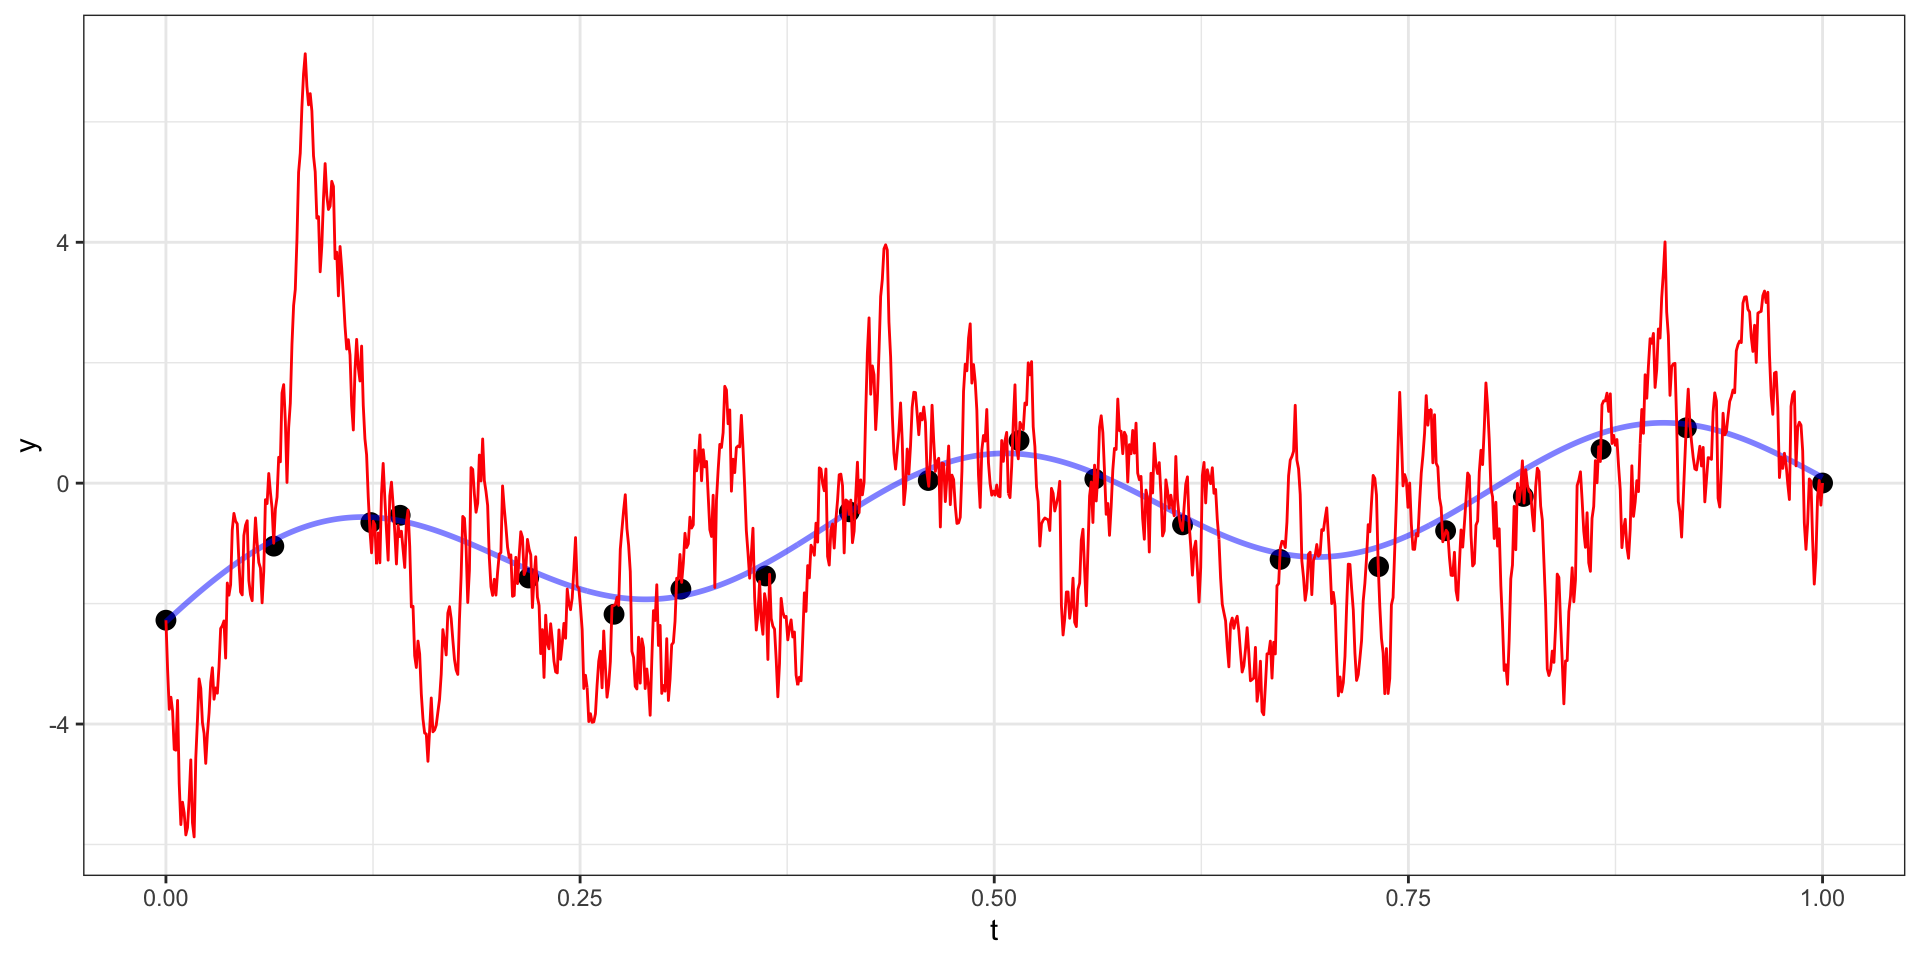
\includegraphics[width=\textwidth]{Lec13_files/figure-beamer/unnamed-chunk-13-1} \end{center}

\begin{verbatim}
## 
## Call:
## lm(formula = pm25 ~ day + I(day^2), data = pm25)
## 
## Coefficients:
## (Intercept)          day     I(day^2)  
##  12.9644351   -0.0724639    0.0001751
## 
## Call:
## lm(formula = pm25 ~ day + I(day^2), data = pm25)
## 
## Coefficients:
## (Intercept)          day     I(day^2)  
##  12.9644351   -0.0724639    0.0001751
\end{verbatim}

\end{frame}

\begin{frame}{Detrended Residuals}
\protect\hypertarget{detrended-residuals}{}

\begin{center}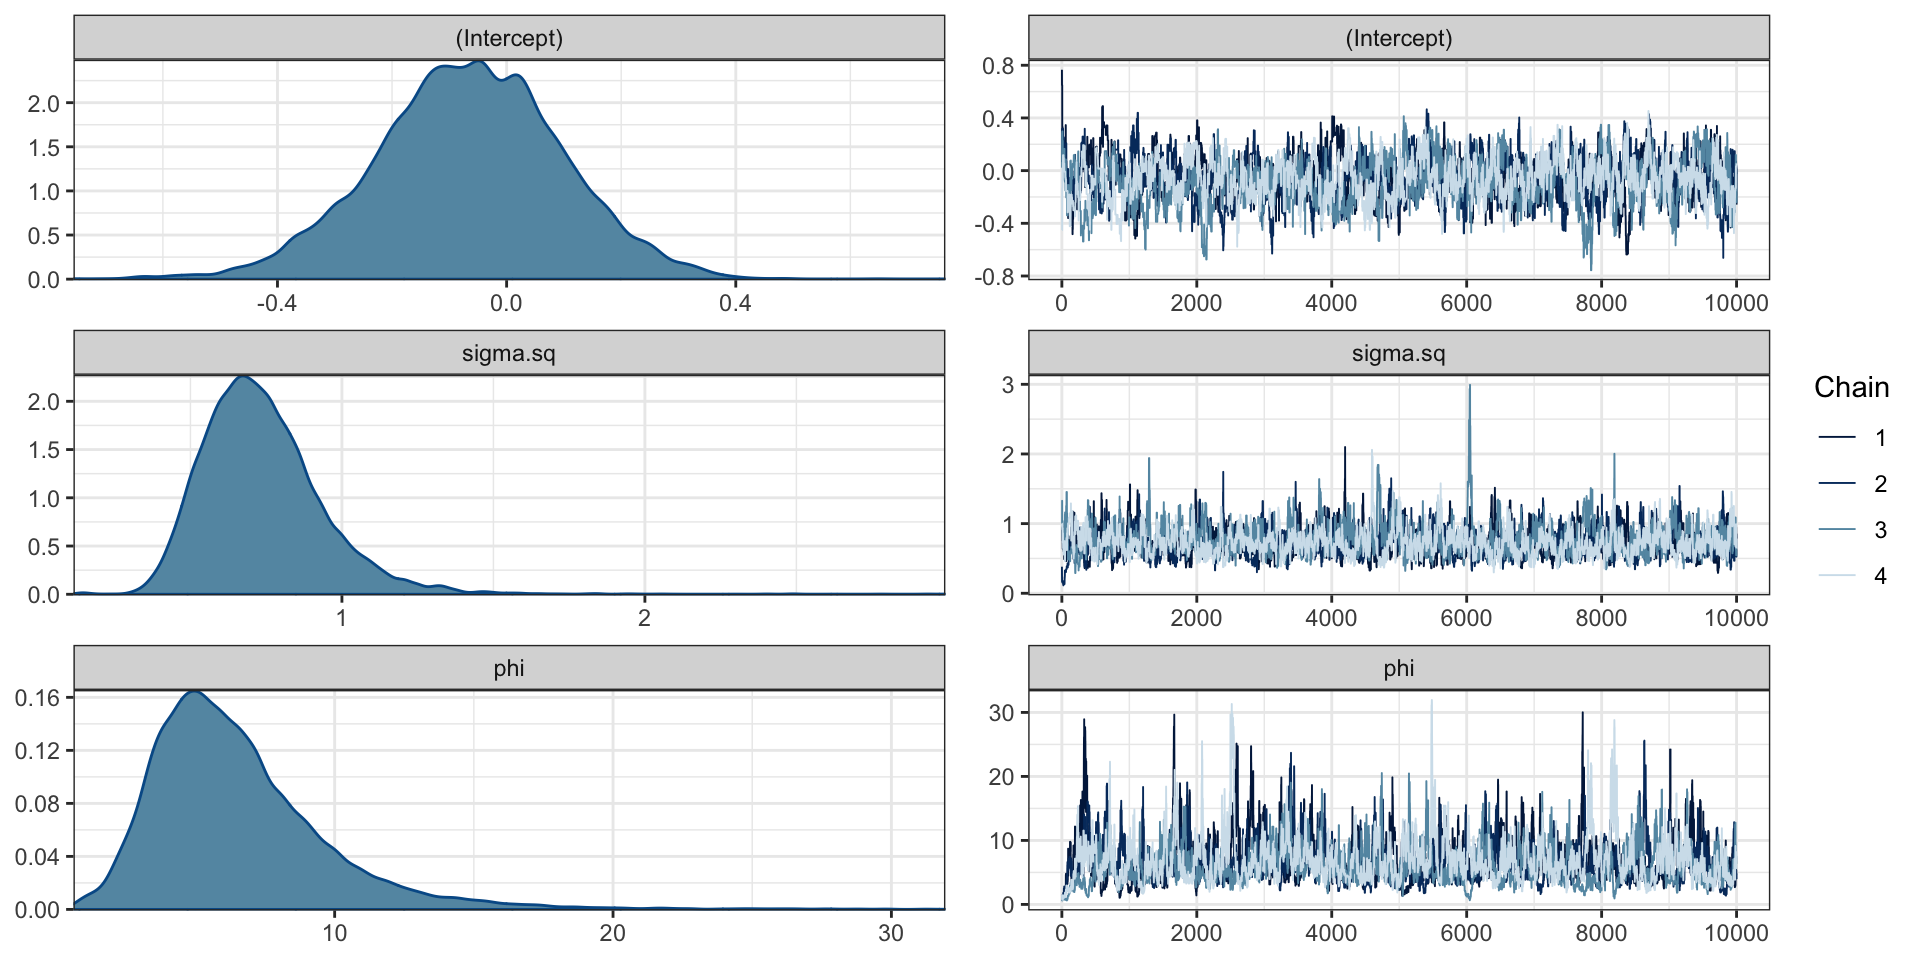
\includegraphics[width=\textwidth]{Lec13_files/figure-beamer/unnamed-chunk-14-1} \end{center}

\end{frame}

\begin{frame}{Empirical Variogram - Residuals}
\protect\hypertarget{empirical-variogram---residuals}{}

\begin{center}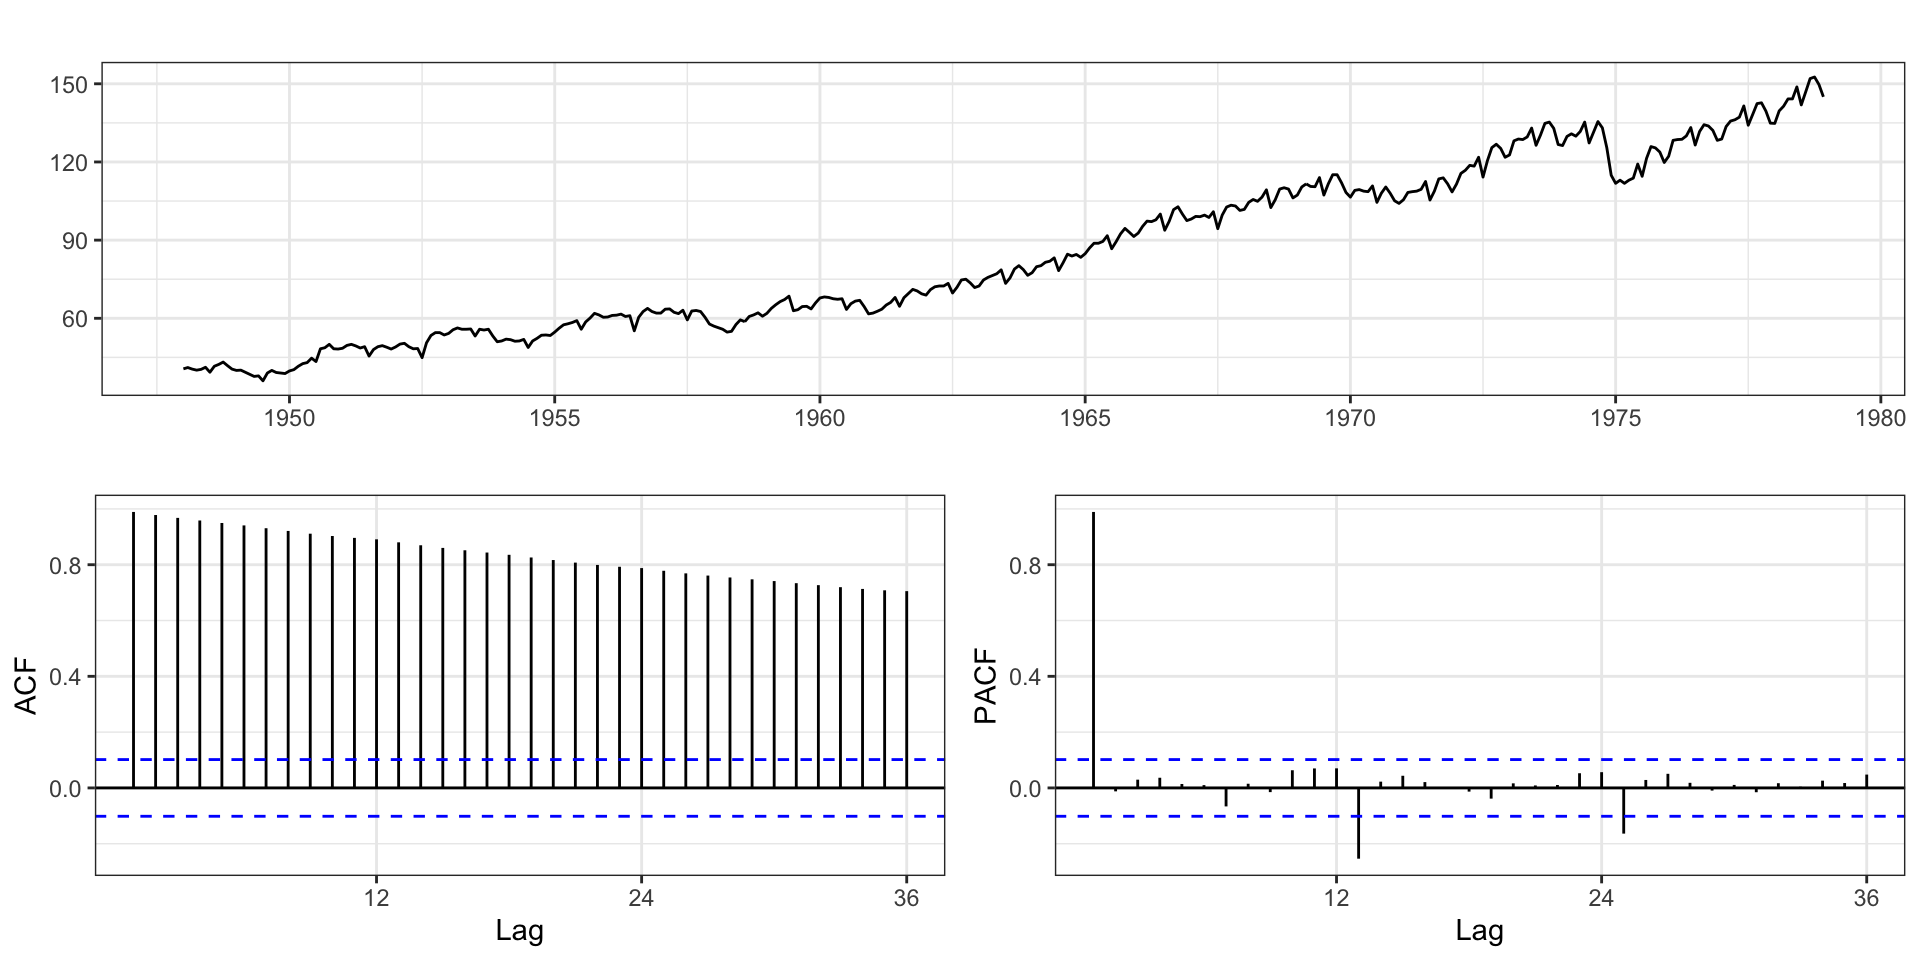
\includegraphics[width=\textwidth]{Lec13_files/figure-beamer/unnamed-chunk-15-1} \end{center}

\end{frame}

\begin{frame}{Zoomed Empirical Variogram - Residuals}
\protect\hypertarget{zoomed-empirical-variogram---residuals}{}

\begin{center}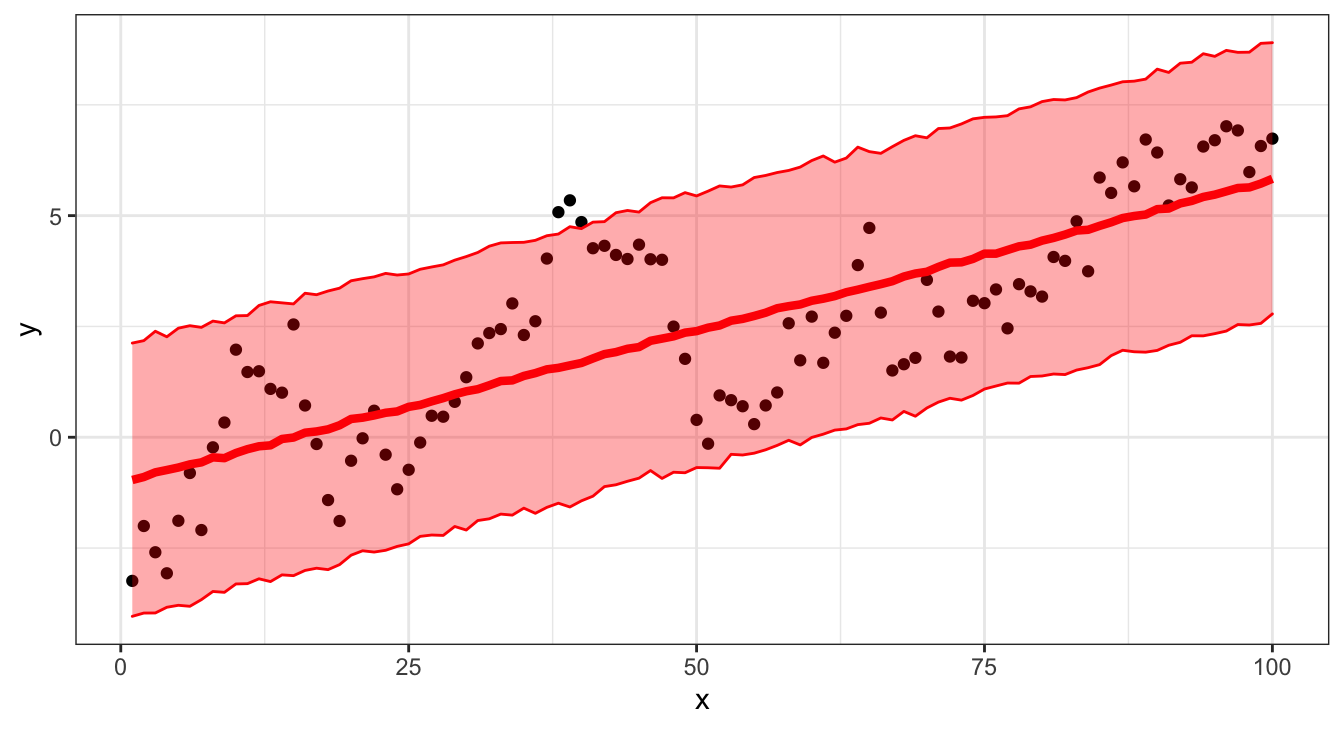
\includegraphics[width=\textwidth]{Lec13_files/figure-beamer/unnamed-chunk-16-1} \end{center}

\end{frame}

\begin{frame}[t]{Model}
\protect\hypertarget{model}{}

What does the model we are trying to fit actually look like?

\pause

\vspace{2mm}

\[ y(t) = \mu(t) + w(t) + \epsilon(t) \] where

\[
\begin{aligned}
\symbf{\mu(t)} &= \beta_0 + \beta_1\, \symbf{t} +\beta_2\, \symbf{t}^2\\
\symbf{w(t)} &\sim \mathcal{GP}(0, \symbf{\Sigma}) \\
\epsilon(t) &\sim \mathcal{N}(0, \sigma^2_w)\\
\\
\{\symbf{\Sigma}\}_{ij} &= Cov(t_i, t_j) =  \sigma^2 \exp(- (|t_i-t_j|\,l)^2)
\end{aligned}
\]

\end{frame}

\begin{frame}[fragile]{JAGS Model}
\protect\hypertarget{jags-model}{}

\scriptoutput

\begin{Shaded}
\begin{Highlighting}[]
\NormalTok{gp_exp_model =}\StringTok{ "model\{}
\StringTok{  y ~ dmnorm(mu, inverse(Sigma))}

\StringTok{  for (i in 1:N) \{}
\StringTok{    mu[i] <- beta[1]+ beta[2] * x[i] + beta[3] * x[i]^2}
\StringTok{  \}}
\StringTok{  }
\StringTok{  for (i in 1:(N-1)) \{}
\StringTok{    for (j in (i+1):N) \{}
\StringTok{      Sigma[i,j] <- sigma2 * exp(- pow(l*d[i,j],2))}
\StringTok{      Sigma[j,i] <- Sigma[i,j]}
\StringTok{    \}}
\StringTok{  \}}

\StringTok{  for (k in 1:N) \{}
\StringTok{    Sigma[k,k] <- sigma2 + sigma2_w}
\StringTok{  \}}

\StringTok{  for (i in 1:3) \{}
\StringTok{    beta[i] ~ dt(coef[i], 2.5, 1)}
\StringTok{  \}}
\StringTok{  sigma2_w ~ dnorm(5, 1/25) T(0,)}
\StringTok{  sigma2   ~ dnorm(12.5, 1/25) T(0,)}
\StringTok{  l        ~ dt(0, 2.5, 1) T(0,) }
\StringTok{\}"}
\end{Highlighting}
\end{Shaded}

\end{frame}

\begin{frame}{Posterior - Betas}
\protect\hypertarget{posterior---betas}{}

\begin{center}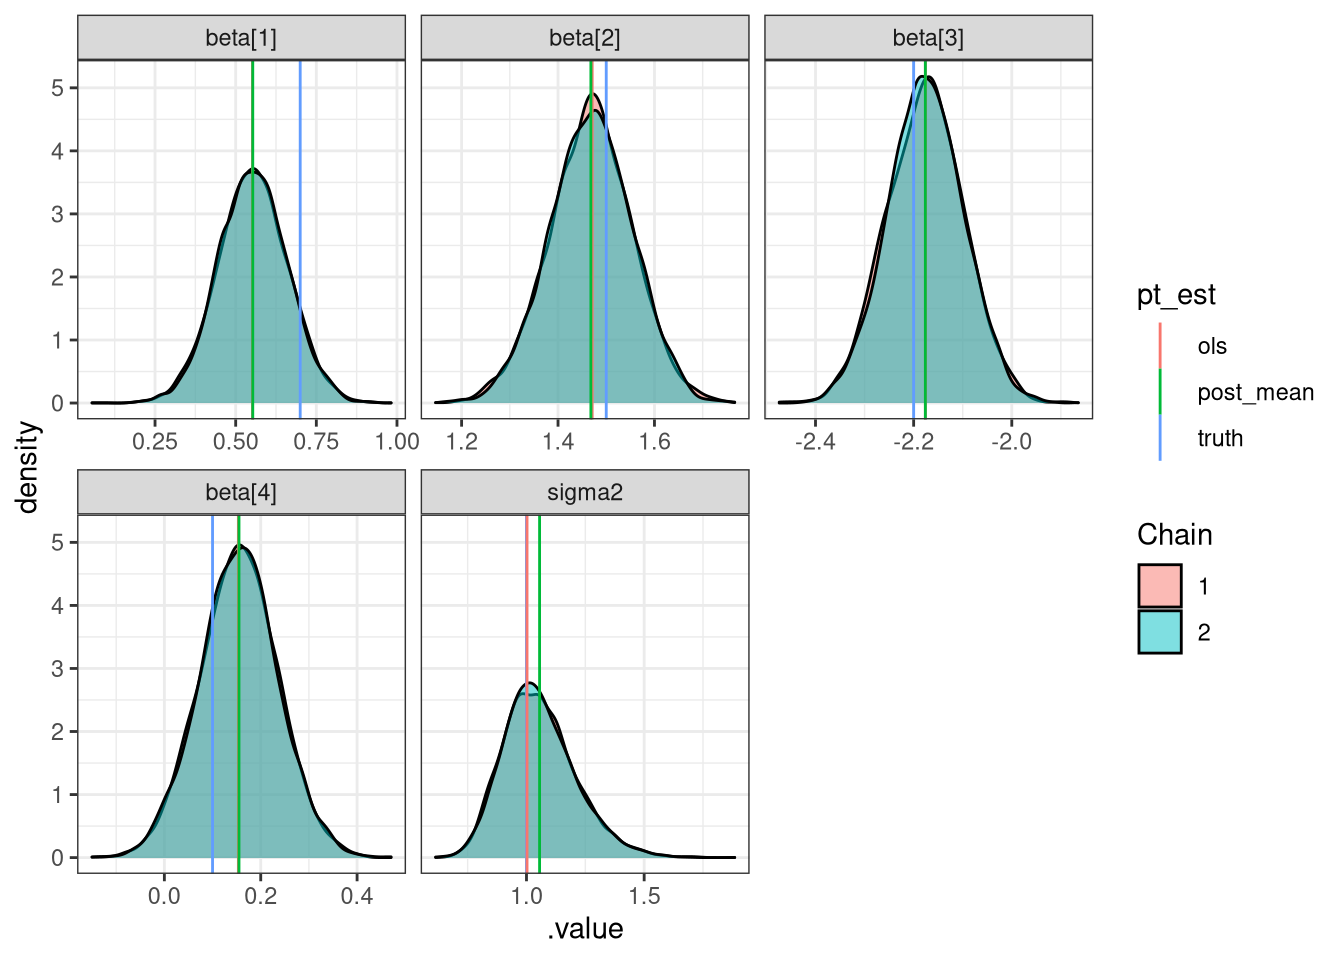
\includegraphics[width=\textwidth]{Lec13_files/figure-beamer/unnamed-chunk-19-1} \end{center}

\end{frame}

\begin{frame}{Posterior - Covariance Parameters}
\protect\hypertarget{posterior---covariance-parameters}{}

\begin{center}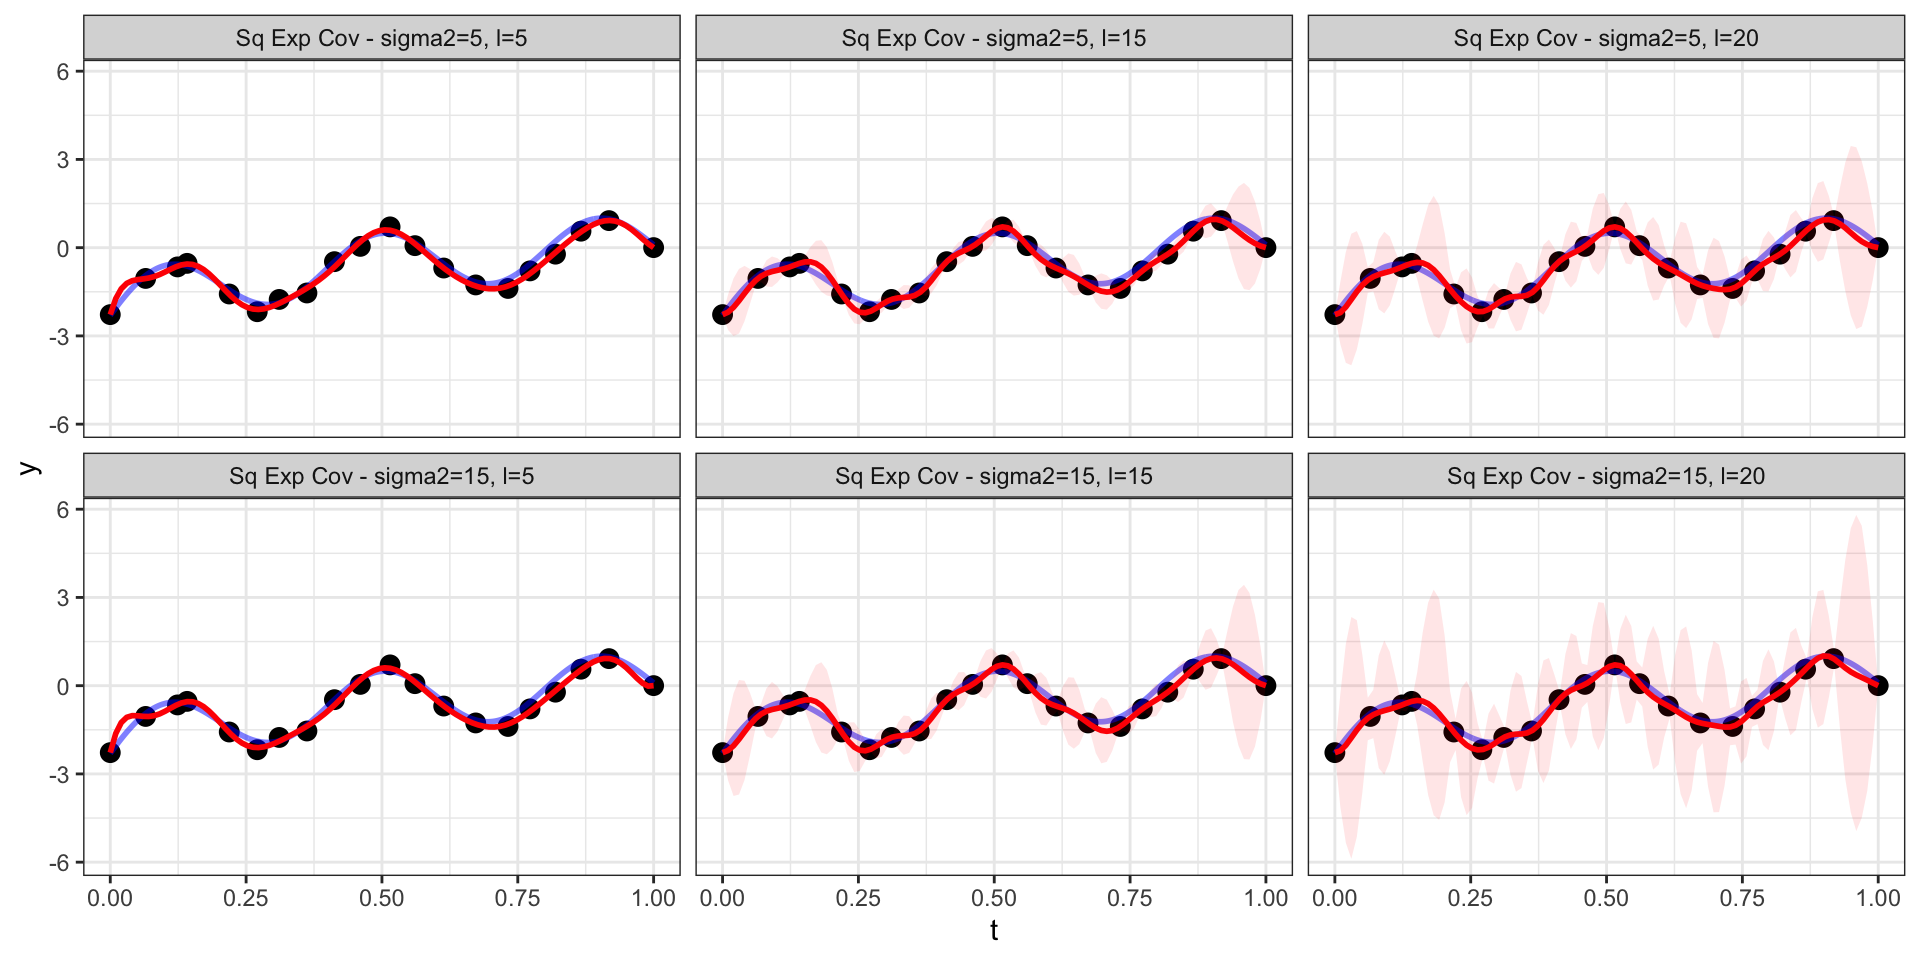
\includegraphics[width=\textwidth]{Lec13_files/figure-beamer/unnamed-chunk-20-1} \end{center}

\end{frame}

\begin{frame}{Posterior - Covariance Parameters}
\protect\hypertarget{posterior---covariance-parameters-1}{}

\begin{center}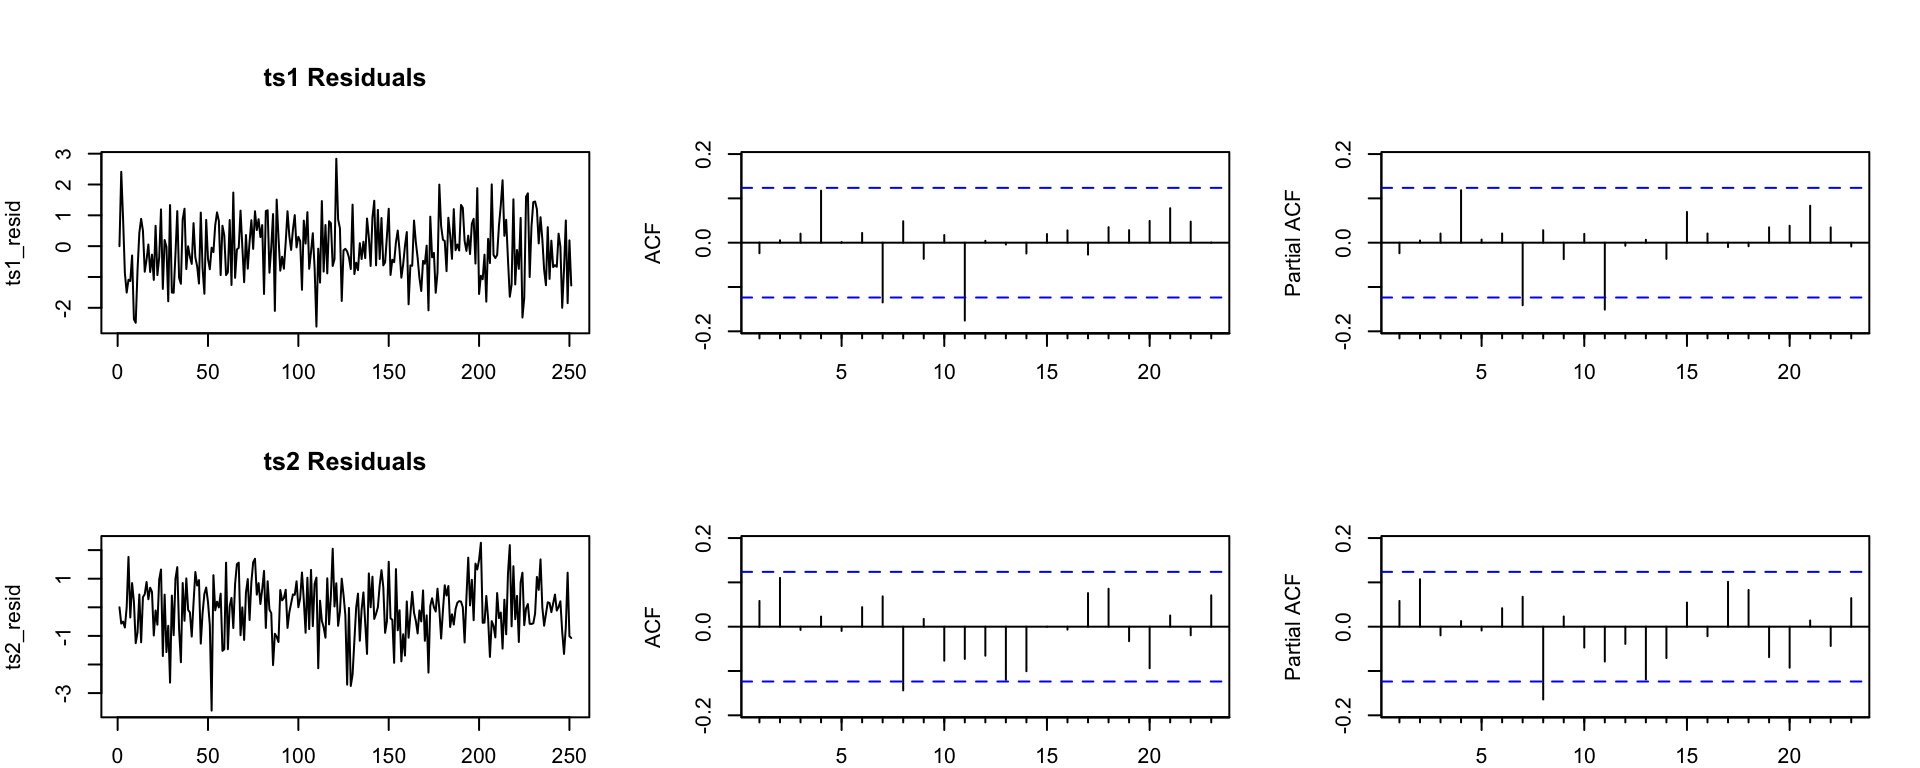
\includegraphics[width=\textwidth]{Lec13_files/figure-beamer/unnamed-chunk-21-1} \end{center}

\end{frame}

\begin{frame}{Posterior - Covariance Parameters - l}
\protect\hypertarget{posterior---covariance-parameters---l}{}

\begin{center}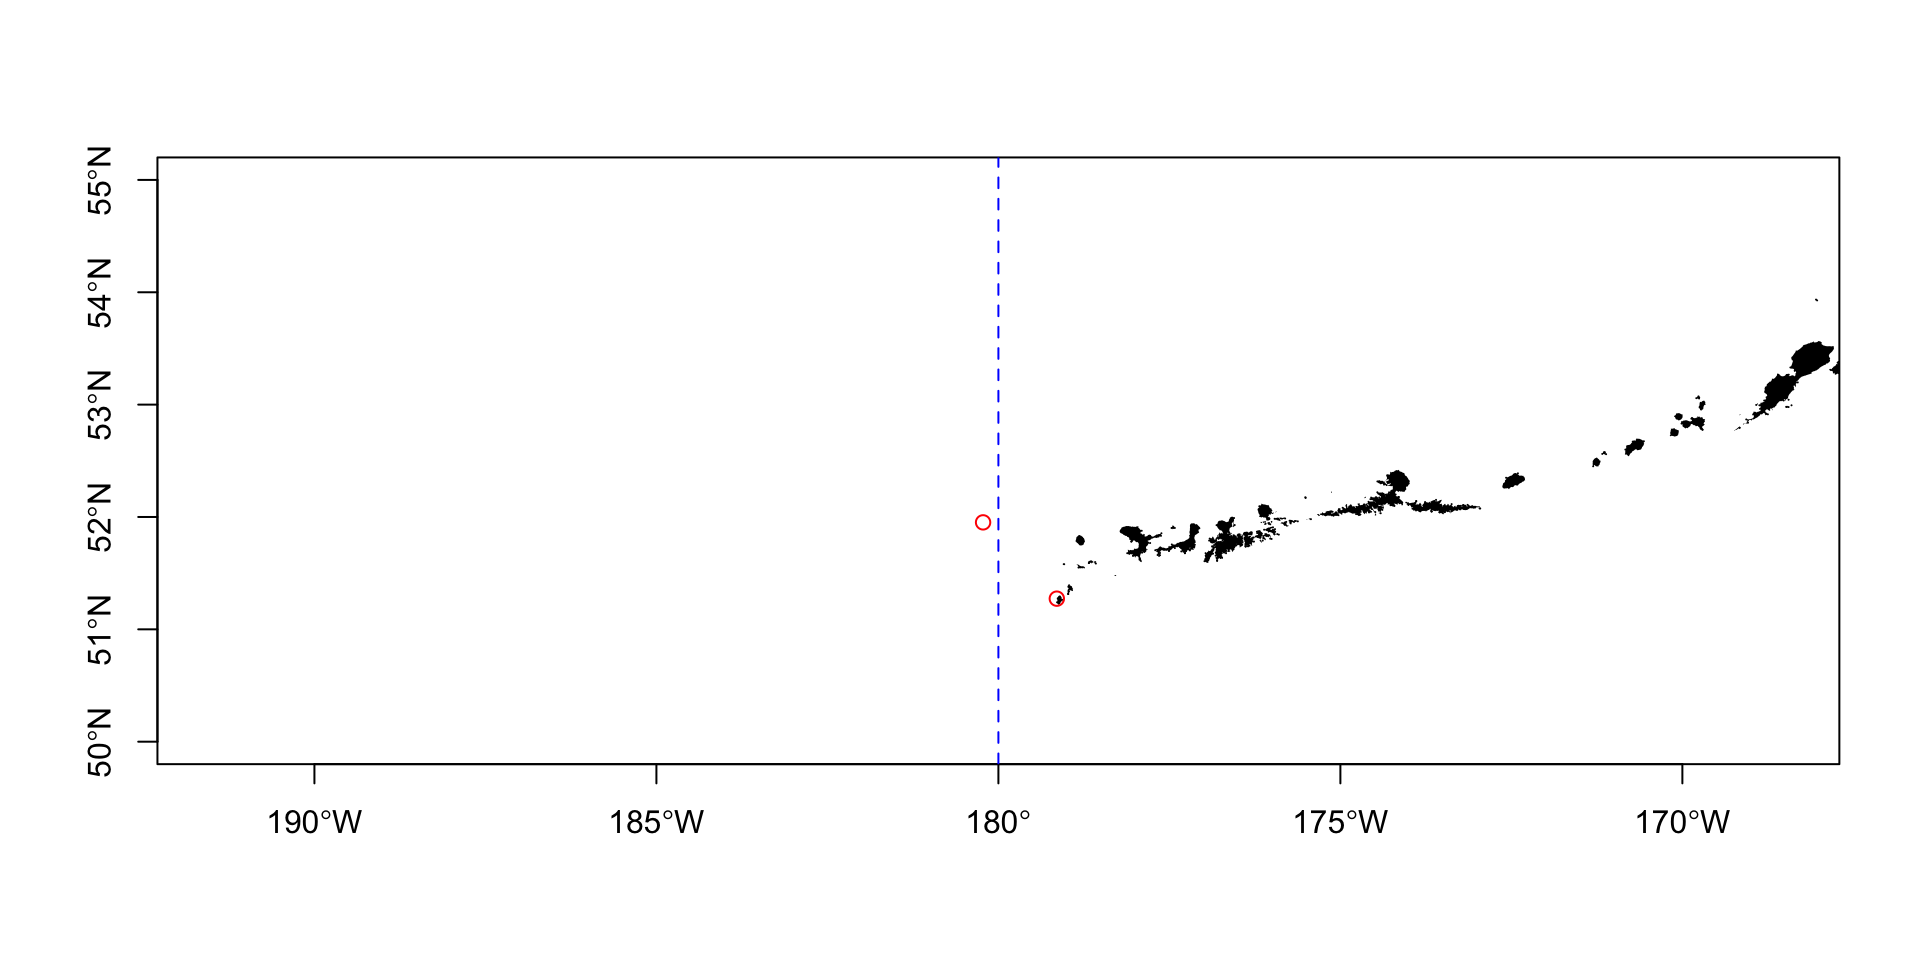
\includegraphics[width=\textwidth]{Lec13_files/figure-beamer/unnamed-chunk-22-1} \end{center}

\end{frame}

\begin{frame}{Posterior}
\protect\hypertarget{posterior}{}

\begin{longtable}[]{@{}lrrrr@{}}
\toprule
.variable & post\_mean & post\_med & post\_lower &
post\_upper\tabularnewline
\midrule
\endhead
beta{[}1{]} & 12.98786 & 12.96919 & 11.52626 & 14.56714\tabularnewline
beta{[}2{]} & -0.07289 & -0.07286 & -0.09259 & -0.05316\tabularnewline
beta{[}3{]} & 0.00018 & 0.00018 & 0.00011 & 0.00023\tabularnewline
l & 5.41433 & 0.86915 & 0.03329 & 52.39913\tabularnewline
sigma2 & 8.87498 & 9.14124 & 2.26513 & 14.62043\tabularnewline
sigma2\_w & 5.25459 & 4.75810 & 0.22093 & 12.52645\tabularnewline
\bottomrule
\end{longtable}

\end{frame}

\begin{frame}{Empirical + Fitted Variogram}
\protect\hypertarget{empirical-fitted-variogram}{}

\begin{center}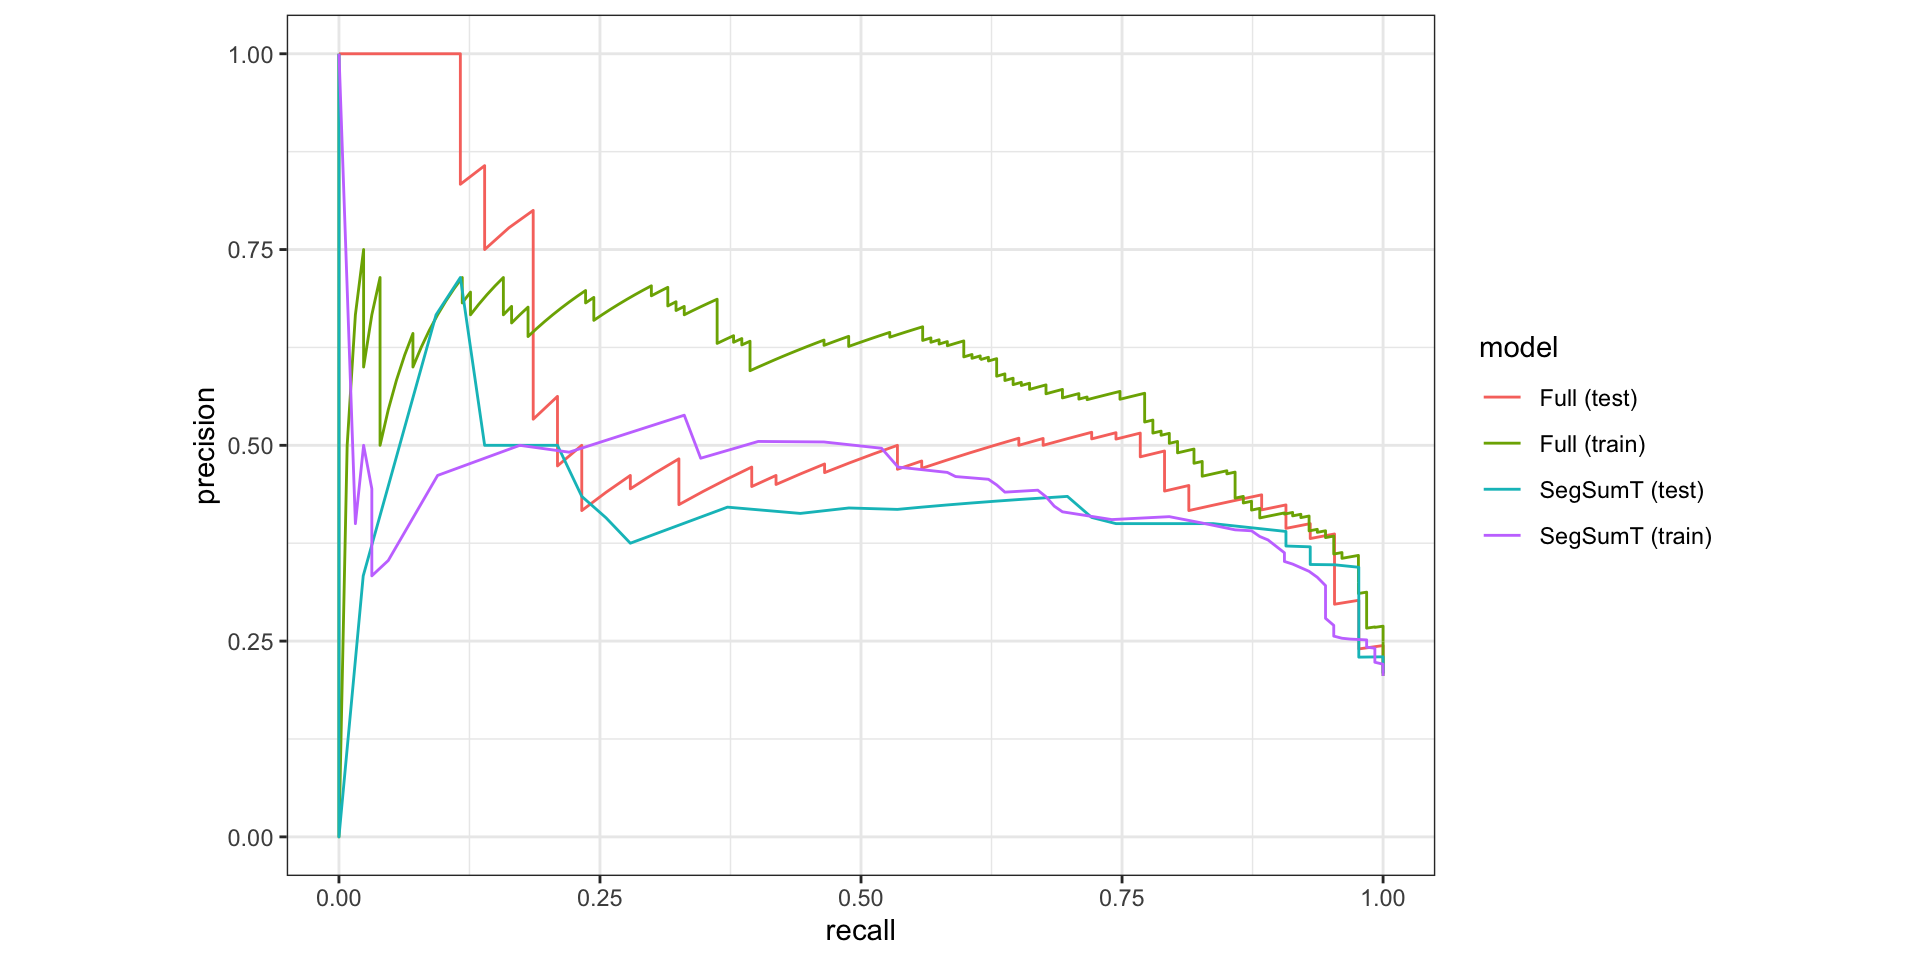
\includegraphics[width=\textwidth]{Lec13_files/figure-beamer/unnamed-chunk-24-1} \end{center}

\end{frame}

\begin{frame}{Fitted Model + Predictions}
\protect\hypertarget{fitted-model-predictions}{}

\begin{center}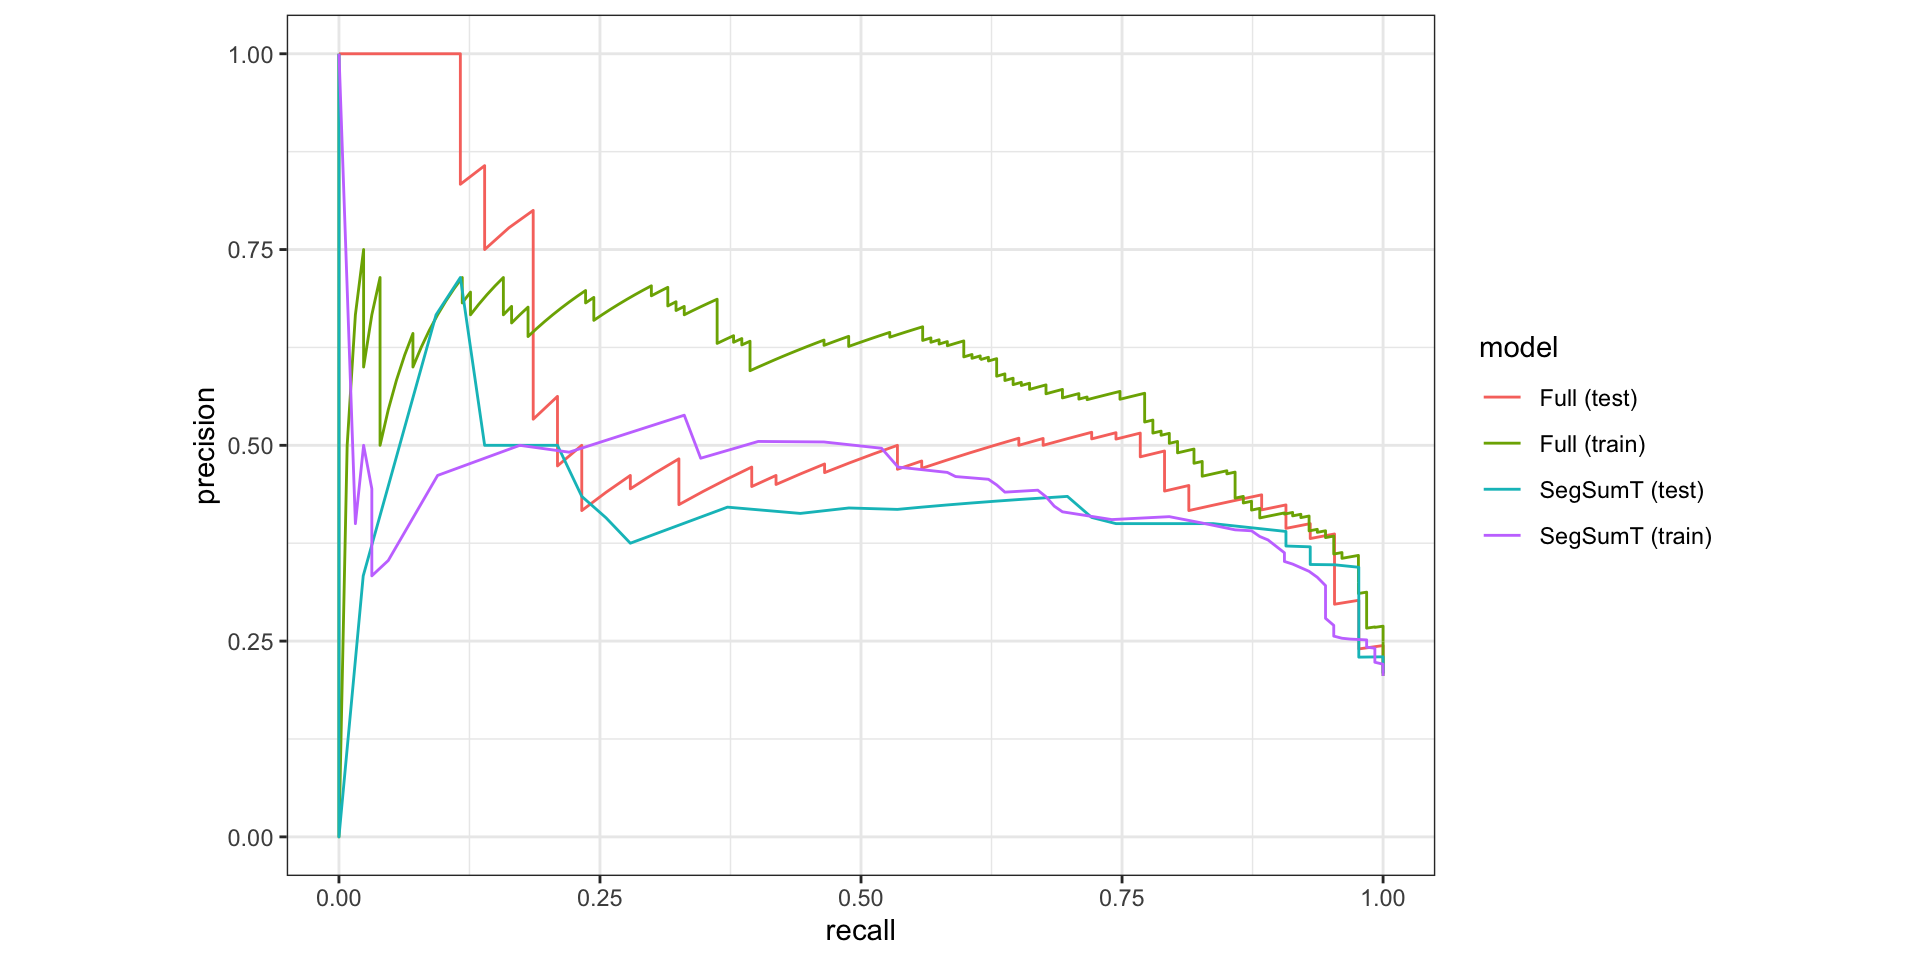
\includegraphics[width=\textwidth]{Lec13_files/figure-beamer/unnamed-chunk-25-1} \end{center}

\end{frame}

\begin{frame}{Empirical Variogram Model}
\protect\hypertarget{empirical-variogram-model}{}

\begin{center}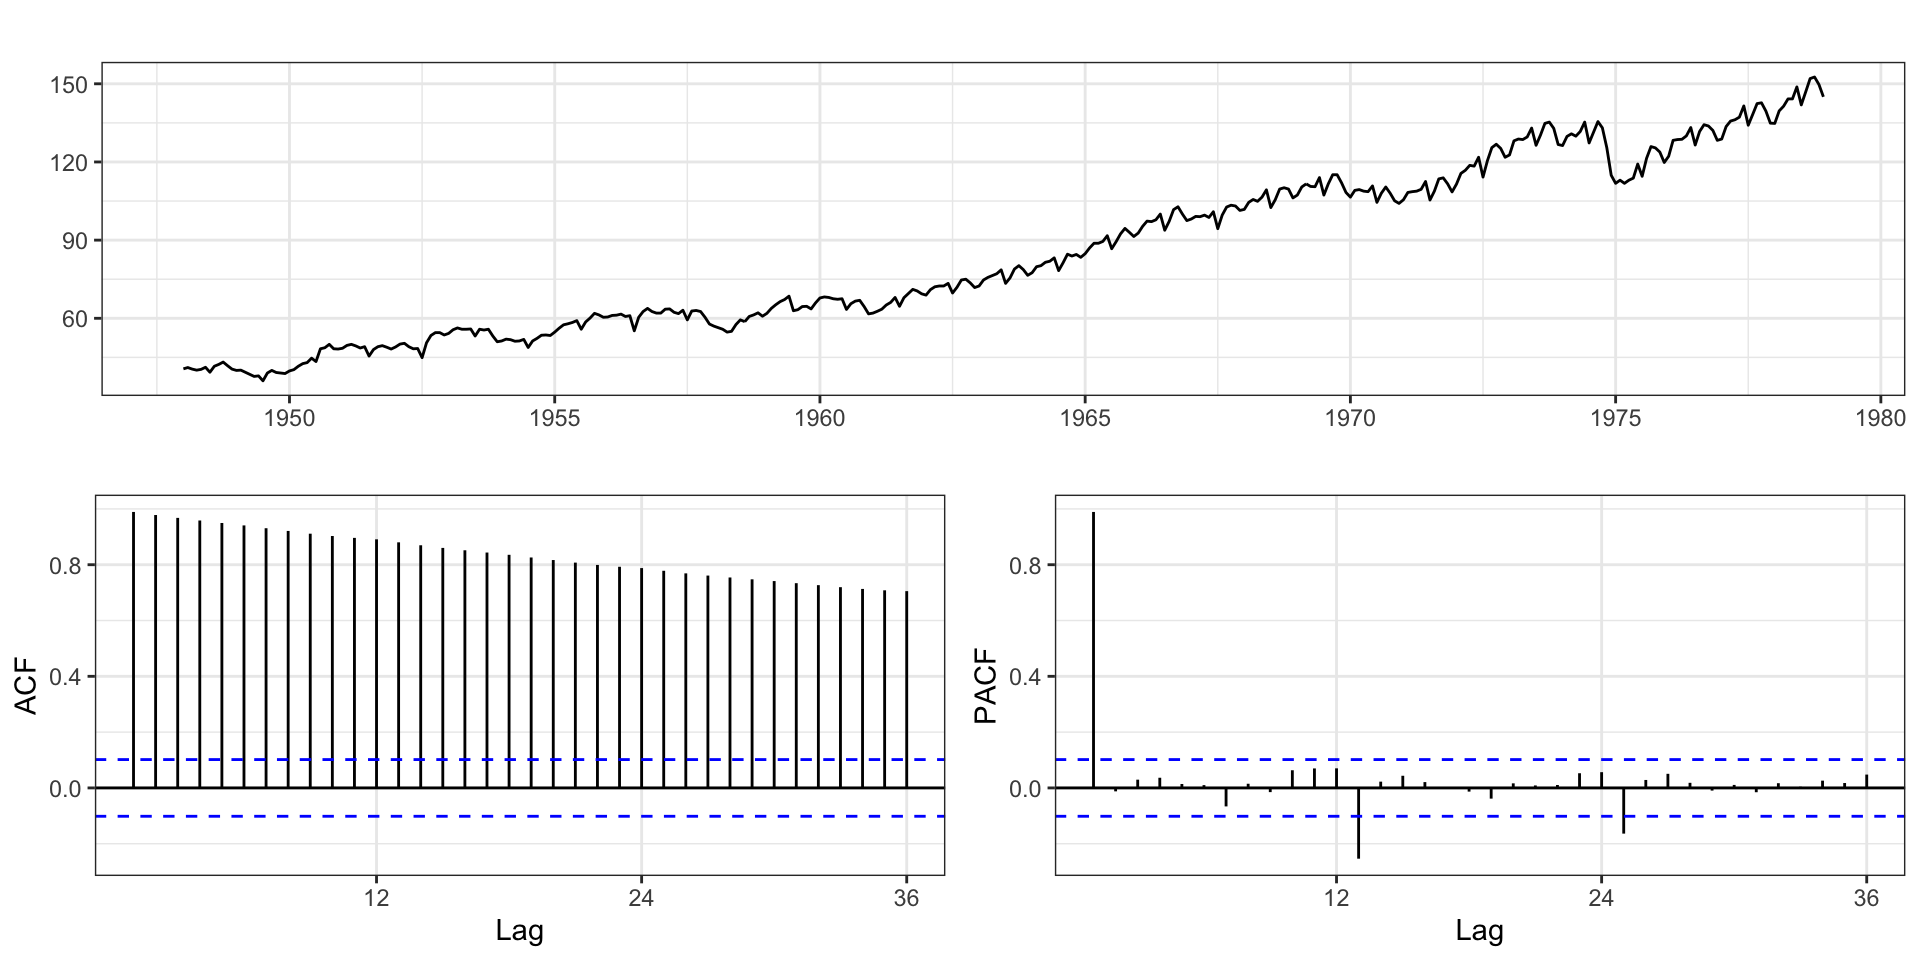
\includegraphics[width=\textwidth]{Lec13_files/figure-beamer/unnamed-chunk-26-1} \end{center}

\end{frame}

\begin{frame}{Fit}
\protect\hypertarget{fit}{}

\begin{center}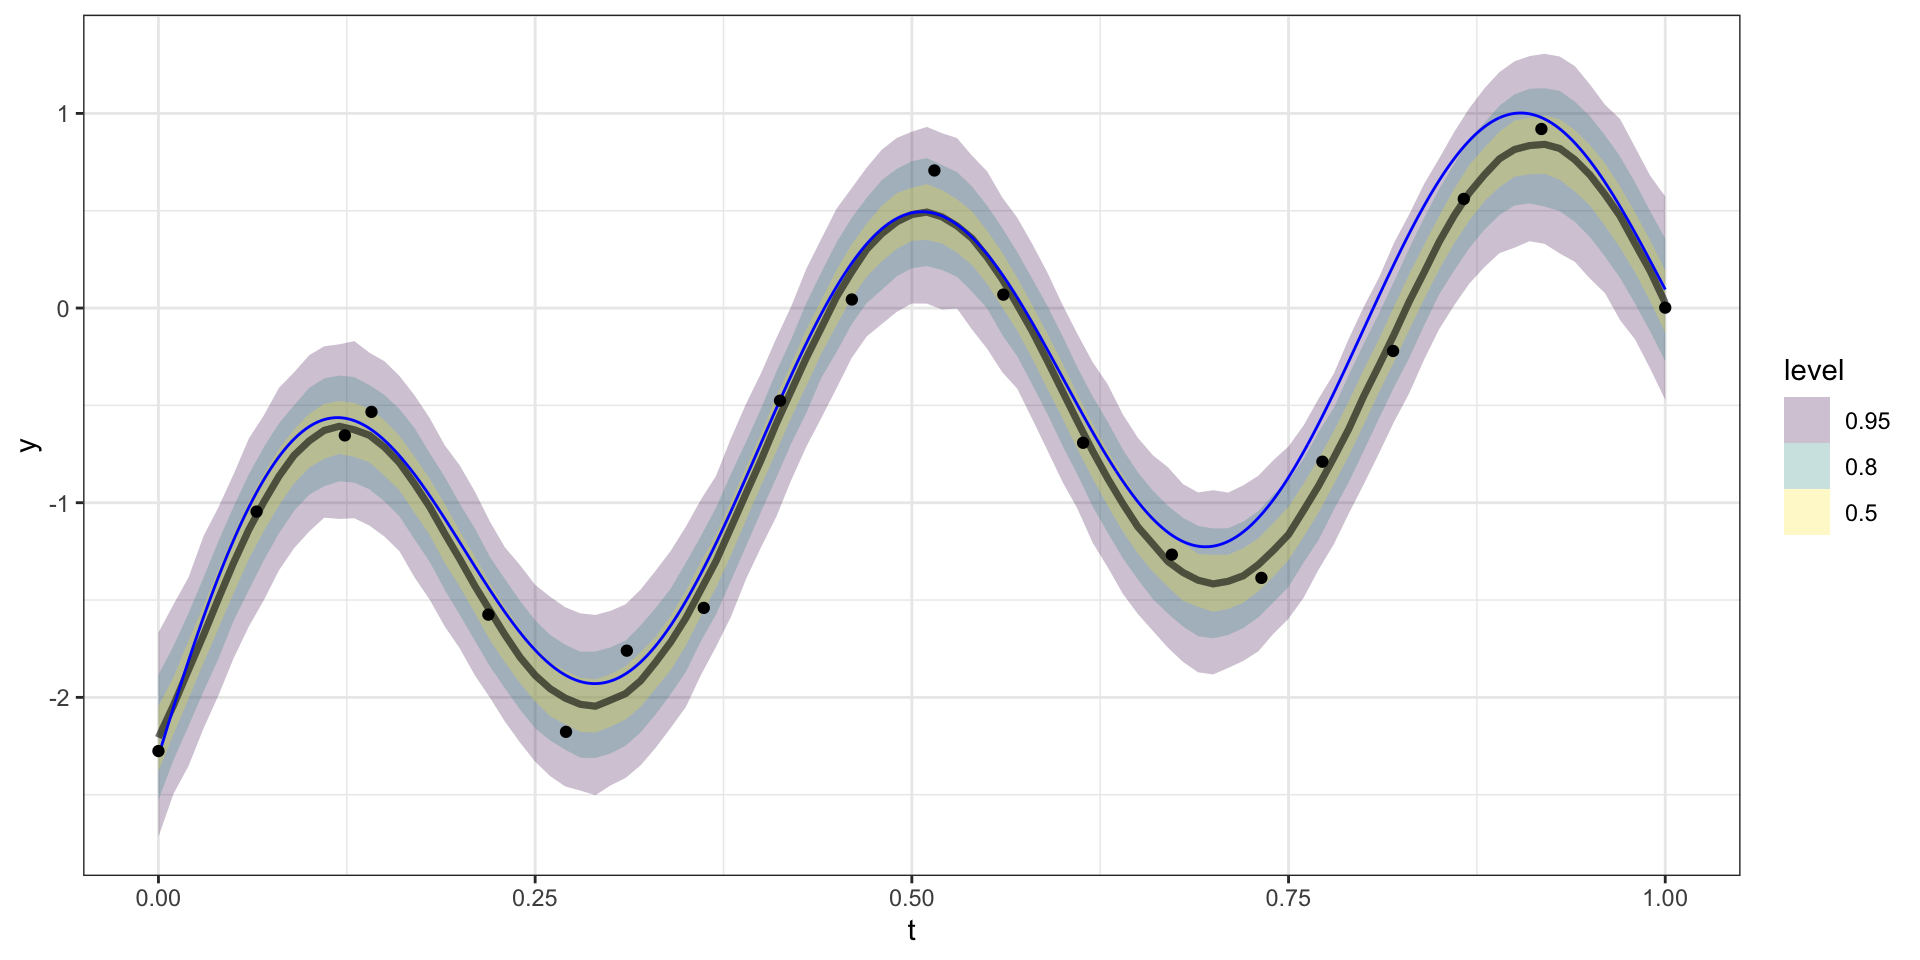
\includegraphics[width=\textwidth]{Lec13_files/figure-beamer/unnamed-chunk-27-1} \end{center}

\end{frame}

\begin{frame}{Predictions}
\protect\hypertarget{predictions}{}

\begin{center}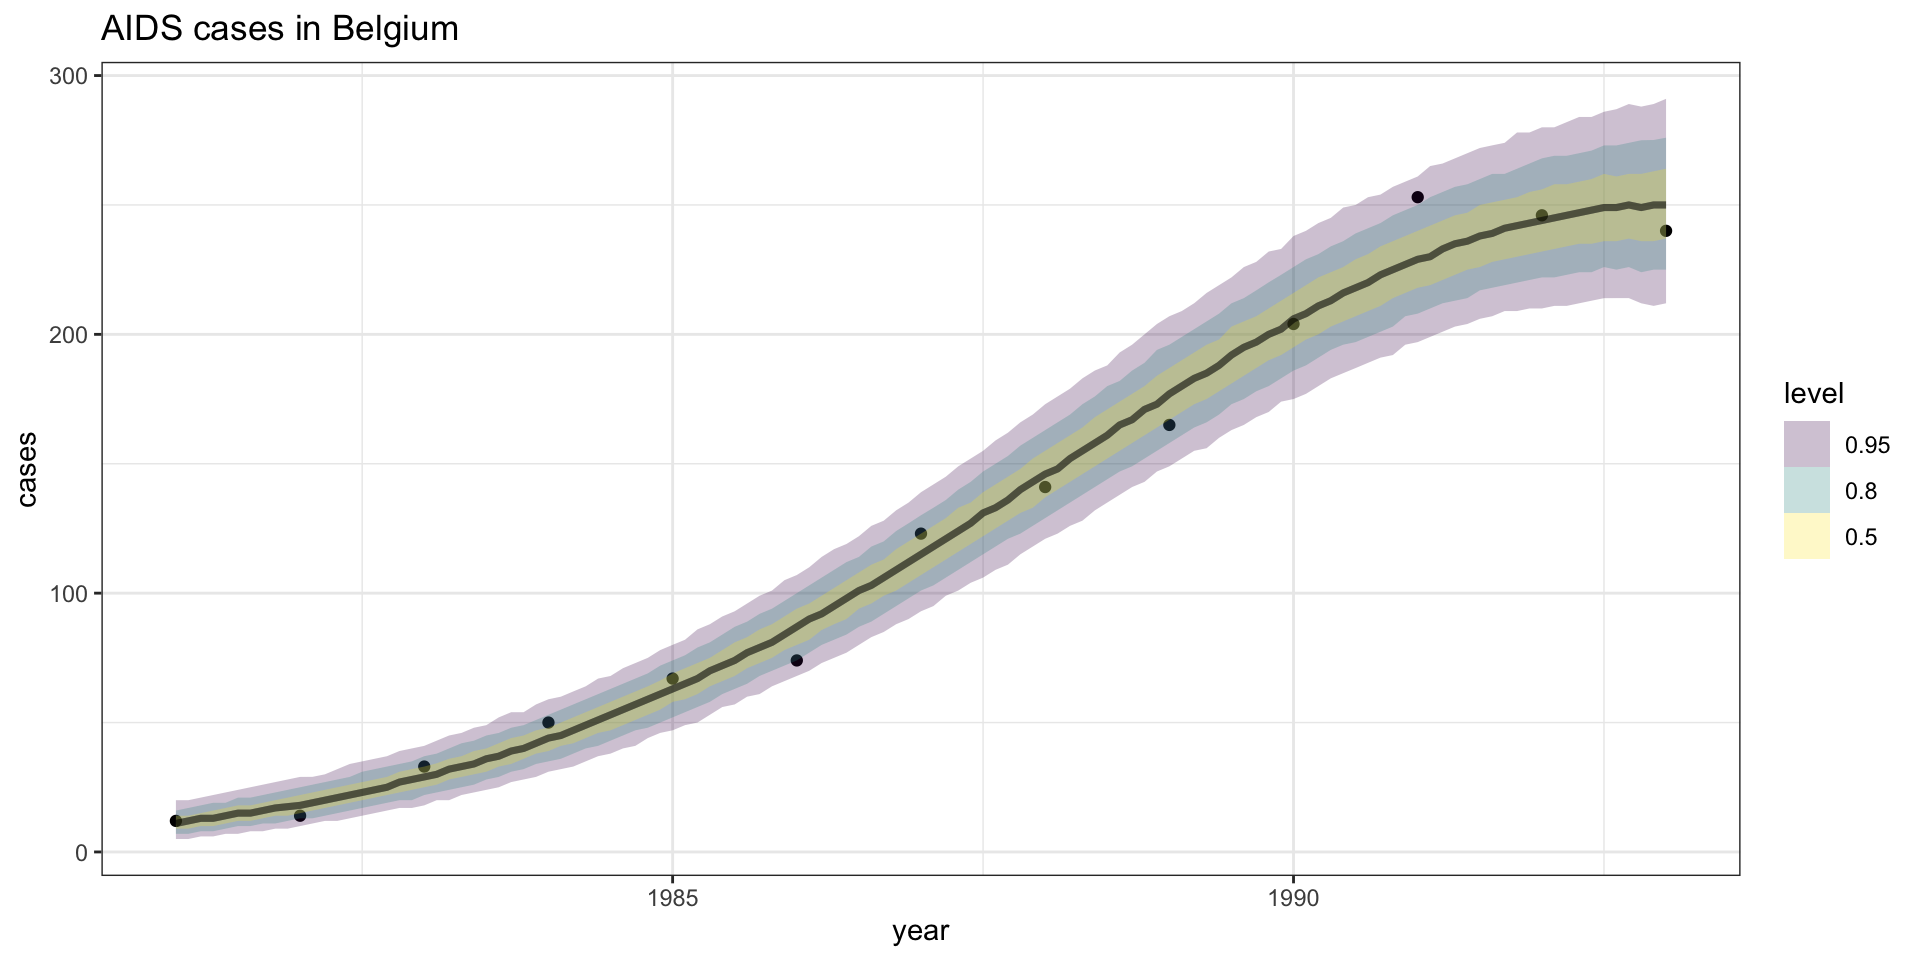
\includegraphics[width=\textwidth]{Lec13_files/figure-beamer/unnamed-chunk-28-1} \end{center}

\end{frame}

\hypertarget{full-posterior-predictive-distribution}{%
\section{Full Posterior Predictive
Distribution}\label{full-posterior-predictive-distribution}}

\begin{frame}[fragile,t]{Plug in Prediction}
\protect\hypertarget{plug-in-prediction}{}

\scriptoutput

\begin{Shaded}
\begin{Highlighting}[]
\NormalTok{l        =}\StringTok{ }\KeywordTok{filter}\NormalTok{(post, .variable }\OperatorTok{==}\StringTok{ 'l'}\NormalTok{)        }\OperatorTok\StringTok{ }\KeywordTok{pull}\NormalTok{(post_med)}
\NormalTok{sigma2   =}\StringTok{ }\KeywordTok{filter}\NormalTok{(post, .variable }\OperatorTok{==}\StringTok{ 'sigma2'}\NormalTok{)   }\OperatorTok\StringTok{ }\KeywordTok{pull}\NormalTok{(post_med)}
\NormalTok{sigma2_w =}\StringTok{ }\KeywordTok{filter}\NormalTok{(post, .variable }\OperatorTok{==}\StringTok{ 'sigma2_w'}\NormalTok{) }\OperatorTok\StringTok{ }\KeywordTok{pull}\NormalTok{(post_med)}
\NormalTok{beta0    =}\StringTok{ }\KeywordTok{filter}\NormalTok{(post, .variable }\OperatorTok{==}\StringTok{ 'beta[1]'}\NormalTok{) }\OperatorTok\StringTok{ }\KeywordTok{pull}\NormalTok{(post_med)}
\NormalTok{beta1    =}\StringTok{ }\KeywordTok{filter}\NormalTok{(post, .variable }\OperatorTok{==}\StringTok{ 'beta[2]'}\NormalTok{) }\OperatorTok\StringTok{ }\KeywordTok{pull}\NormalTok{(post_med)}
\NormalTok{beta2    =}\StringTok{ }\KeywordTok{filter}\NormalTok{(post, .variable }\OperatorTok{==}\StringTok{ 'beta[3]'}\NormalTok{) }\OperatorTok\StringTok{ }\KeywordTok{pull}\NormalTok{(post_med)}
   
\NormalTok{reps=}\DecValTok{1000}

\NormalTok{x =}\StringTok{ }\NormalTok{pm25}\OperatorTok{$}\NormalTok{day}
\NormalTok{y =}\StringTok{ }\NormalTok{pm25}\OperatorTok{$}\NormalTok{pm25}
\NormalTok{x_pred =}\StringTok{ }\DecValTok{1}\OperatorTok{:}\DecValTok{365} \OperatorTok{+}\StringTok{ }\KeywordTok{rnorm}\NormalTok{(}\DecValTok{365}\NormalTok{, }\FloatTok{0.01}\NormalTok{)}

\NormalTok{mu =}\StringTok{ }\NormalTok{beta0 }\OperatorTok{+}\StringTok{ }\NormalTok{beta1}\OperatorTok{*}\NormalTok{x }\OperatorTok{+}\StringTok{ }\NormalTok{beta2}\OperatorTok{*}\NormalTok{x}\OperatorTok{^}\DecValTok{2}
\NormalTok{mu_pred =}\StringTok{ }\NormalTok{beta0 }\OperatorTok{+}\StringTok{ }\NormalTok{beta1}\OperatorTok{*}\NormalTok{x_pred }\OperatorTok{+}\StringTok{ }\NormalTok{beta2}\OperatorTok{*}\NormalTok{x_pred}\OperatorTok{^}\DecValTok{2}

\NormalTok{dist_o =}\StringTok{ }\NormalTok{fields}\OperatorTok{::}\KeywordTok{rdist}\NormalTok{(x)}
\NormalTok{dist_p =}\StringTok{ }\NormalTok{fields}\OperatorTok{::}\KeywordTok{rdist}\NormalTok{(x_pred)}
\NormalTok{dist_op =}\StringTok{ }\NormalTok{fields}\OperatorTok{::}\KeywordTok{rdist}\NormalTok{(x, x_pred)}
\NormalTok{dist_po =}\StringTok{ }\KeywordTok{t}\NormalTok{(dist_op)}
  
\NormalTok{cov_o  =}\StringTok{ }\KeywordTok{sq_exp_cov}\NormalTok{(dist_o,  }\DataTypeTok{sigma2 =}\NormalTok{ sigma2, }\DataTypeTok{l =}\NormalTok{ l) }\OperatorTok{+}\StringTok{ }\KeywordTok{nugget_cov}\NormalTok{(dist_o, }\DataTypeTok{sigma2 =}\NormalTok{ sigma2_w)}
\NormalTok{cov_p  =}\StringTok{ }\KeywordTok{sq_exp_cov}\NormalTok{(dist_p,  }\DataTypeTok{sigma2 =}\NormalTok{ sigma2, }\DataTypeTok{l =}\NormalTok{ l) }\OperatorTok{+}\StringTok{ }\KeywordTok{nugget_cov}\NormalTok{(dist_p, }\DataTypeTok{sigma2 =}\NormalTok{ sigma2_w)}
\NormalTok{cov_op =}\StringTok{ }\KeywordTok{sq_exp_cov}\NormalTok{(dist_op, }\DataTypeTok{sigma2 =}\NormalTok{ sigma2, }\DataTypeTok{l =}\NormalTok{ l) }\OperatorTok{+}\StringTok{ }\KeywordTok{nugget_cov}\NormalTok{(dist_op, }\DataTypeTok{sigma2 =}\NormalTok{ sigma2_w)}
\NormalTok{cov_po =}\StringTok{ }\KeywordTok{sq_exp_cov}\NormalTok{(dist_po, }\DataTypeTok{sigma2 =}\NormalTok{ sigma2, }\DataTypeTok{l =}\NormalTok{ l) }\OperatorTok{+}\StringTok{ }\KeywordTok{nugget_cov}\NormalTok{(dist_po, }\DataTypeTok{sigma2 =}\NormalTok{ sigma2_w)}

\NormalTok{inv =}\StringTok{ }\KeywordTok{solve}\NormalTok{(cov_o, cov_op)}
\NormalTok{cond_cov =}\StringTok{ }\NormalTok{cov_p }\OperatorTok{-}\StringTok{ }\NormalTok{cov_po }\OperatorTok\StringTok{ }\NormalTok{inv}
\NormalTok{cond_mu  =}\StringTok{ }\NormalTok{mu_pred }\OperatorTok{+}\StringTok{ }\KeywordTok{t}\NormalTok{(inv) }\OperatorTok\StringTok{ }\NormalTok{(y }\OperatorTok{-}\StringTok{ }\NormalTok{mu)}
  
\NormalTok{pred =}\StringTok{ }\NormalTok{cond_mu }\OperatorTok\StringTok{ }\KeywordTok{matrix}\NormalTok{(}\DecValTok{1}\NormalTok{, }\DataTypeTok{ncol=}\NormalTok{reps) }\OperatorTok{+}\StringTok{ }\KeywordTok{t}\NormalTok{(}\KeywordTok{chol}\NormalTok{(cond_cov)) }\OperatorTok\StringTok{ }\KeywordTok{matrix}\NormalTok{(}\KeywordTok{rnorm}\NormalTok{(}\KeywordTok{length}\NormalTok{(x_pred)}\OperatorTok{*}\NormalTok{reps), }\DataTypeTok{ncol=}\NormalTok{reps)}
\end{Highlighting}
\end{Shaded}

\end{frame}

\begin{frame}[t]{Full Posterior Predictive Distribution}
\protect\hypertarget{full-posterior-predictive-distribution-1}{}

Our posterior consists of samples from
\[ l, \sigma^2, \sigma^2_w, \beta_0, \beta_1, \beta_2 ~|~ \symbf{y} \]

and for the purposes of generating the posterior predictions we sampled
\[ \symbf{y}_{pred} ~|~ l^{(m)}, {\sigma^2}^{(m)}, {\sigma^2_w}^{(m)}, {\beta_0}^{(m)}, {\beta_1}^{(m)}, {\beta_2}^{(m)}, \symbf{y} \]
where \(l^{(m)}, \ldots, {\beta_2}^{(m)}\), etc. are the posterior
median of that parameter.

\pause

\vspace{5mm}

In practice we should instead be sampling

\[ \symbf{y}^{(i)}_{pred} ~|~ l^{(i)}, {\sigma^2}^{(i)}, {\sigma^2_w}^{(i)}, {\beta_0}^{(i)}, {\beta_1}^{(i)}, {\beta_2}^{(i)}, \symbf{y} \]
since this takes into account the additional uncertainty in the model
parameters.

\end{frame}

\begin{frame}{Full Posterior Predictive Distribution - Plots}
\protect\hypertarget{full-posterior-predictive-distribution---plots}{}

\begin{center}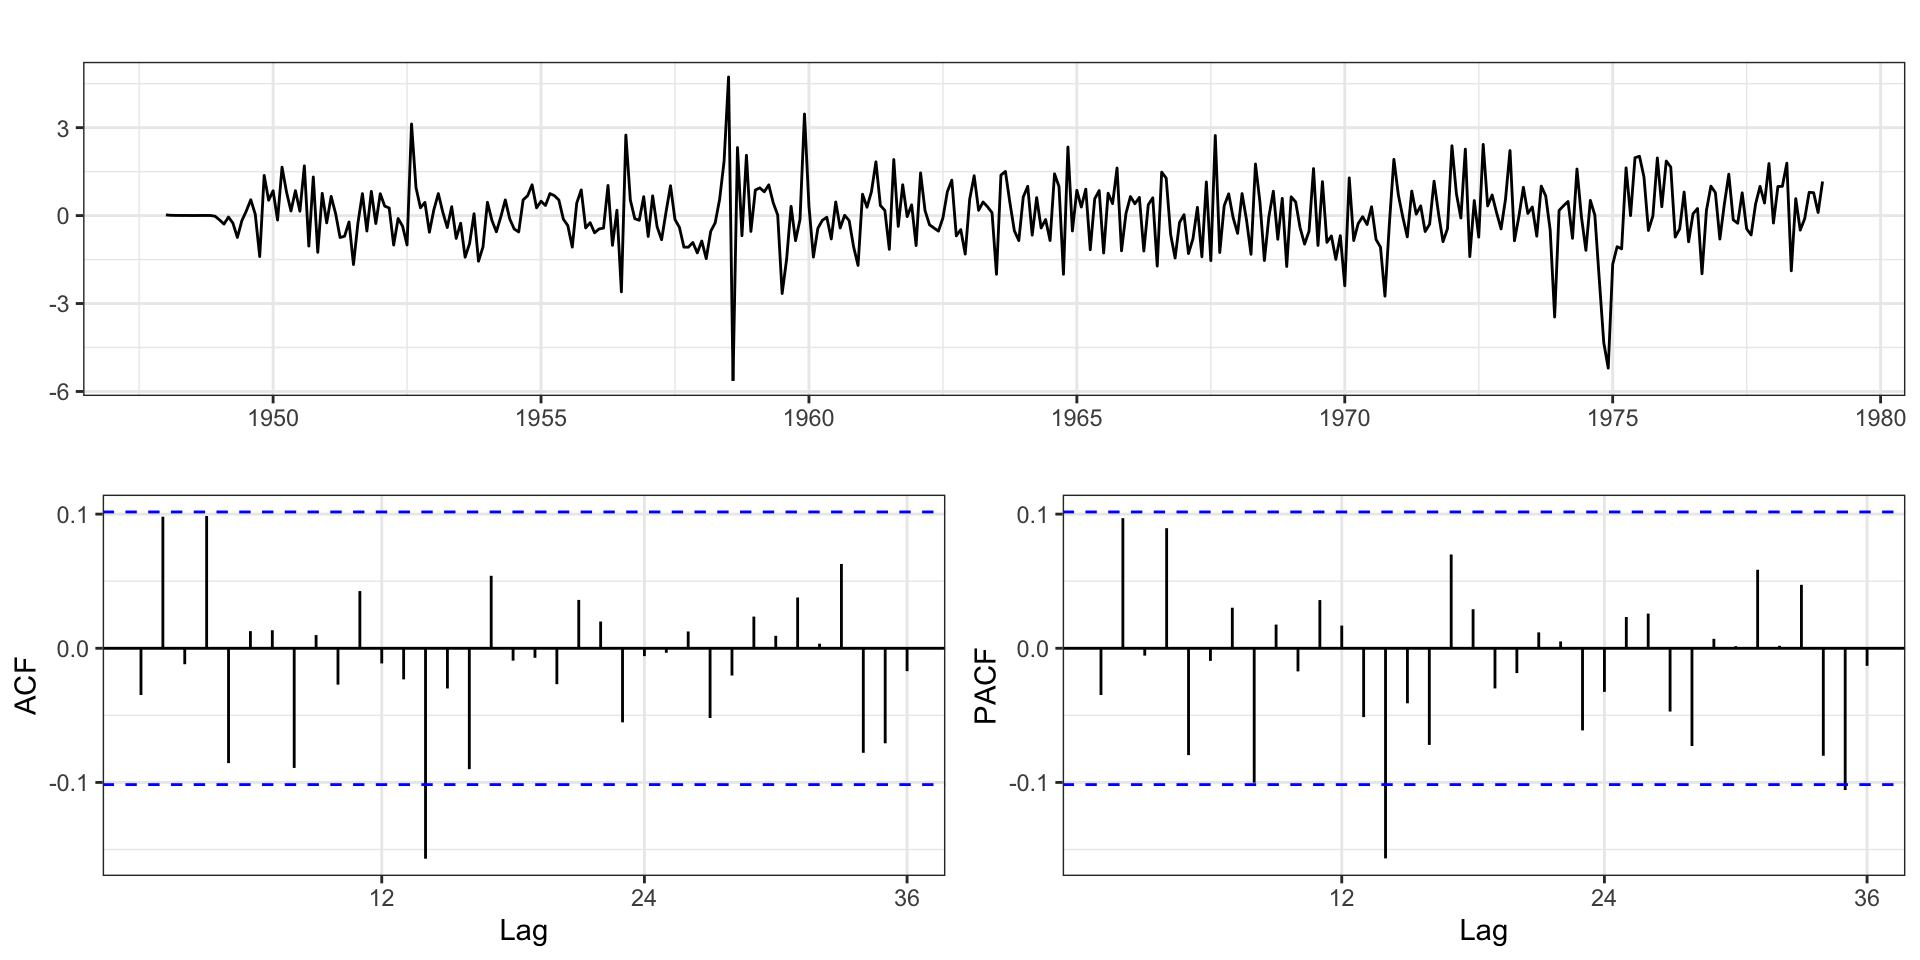
\includegraphics[width=\textwidth]{Lec13_files/figure-beamer/unnamed-chunk-31-1} \end{center}

\end{frame}

\begin{frame}{Full Posterior Predictive Distribution - Median + CI}
\protect\hypertarget{full-posterior-predictive-distribution---median-ci}{}

\begin{center}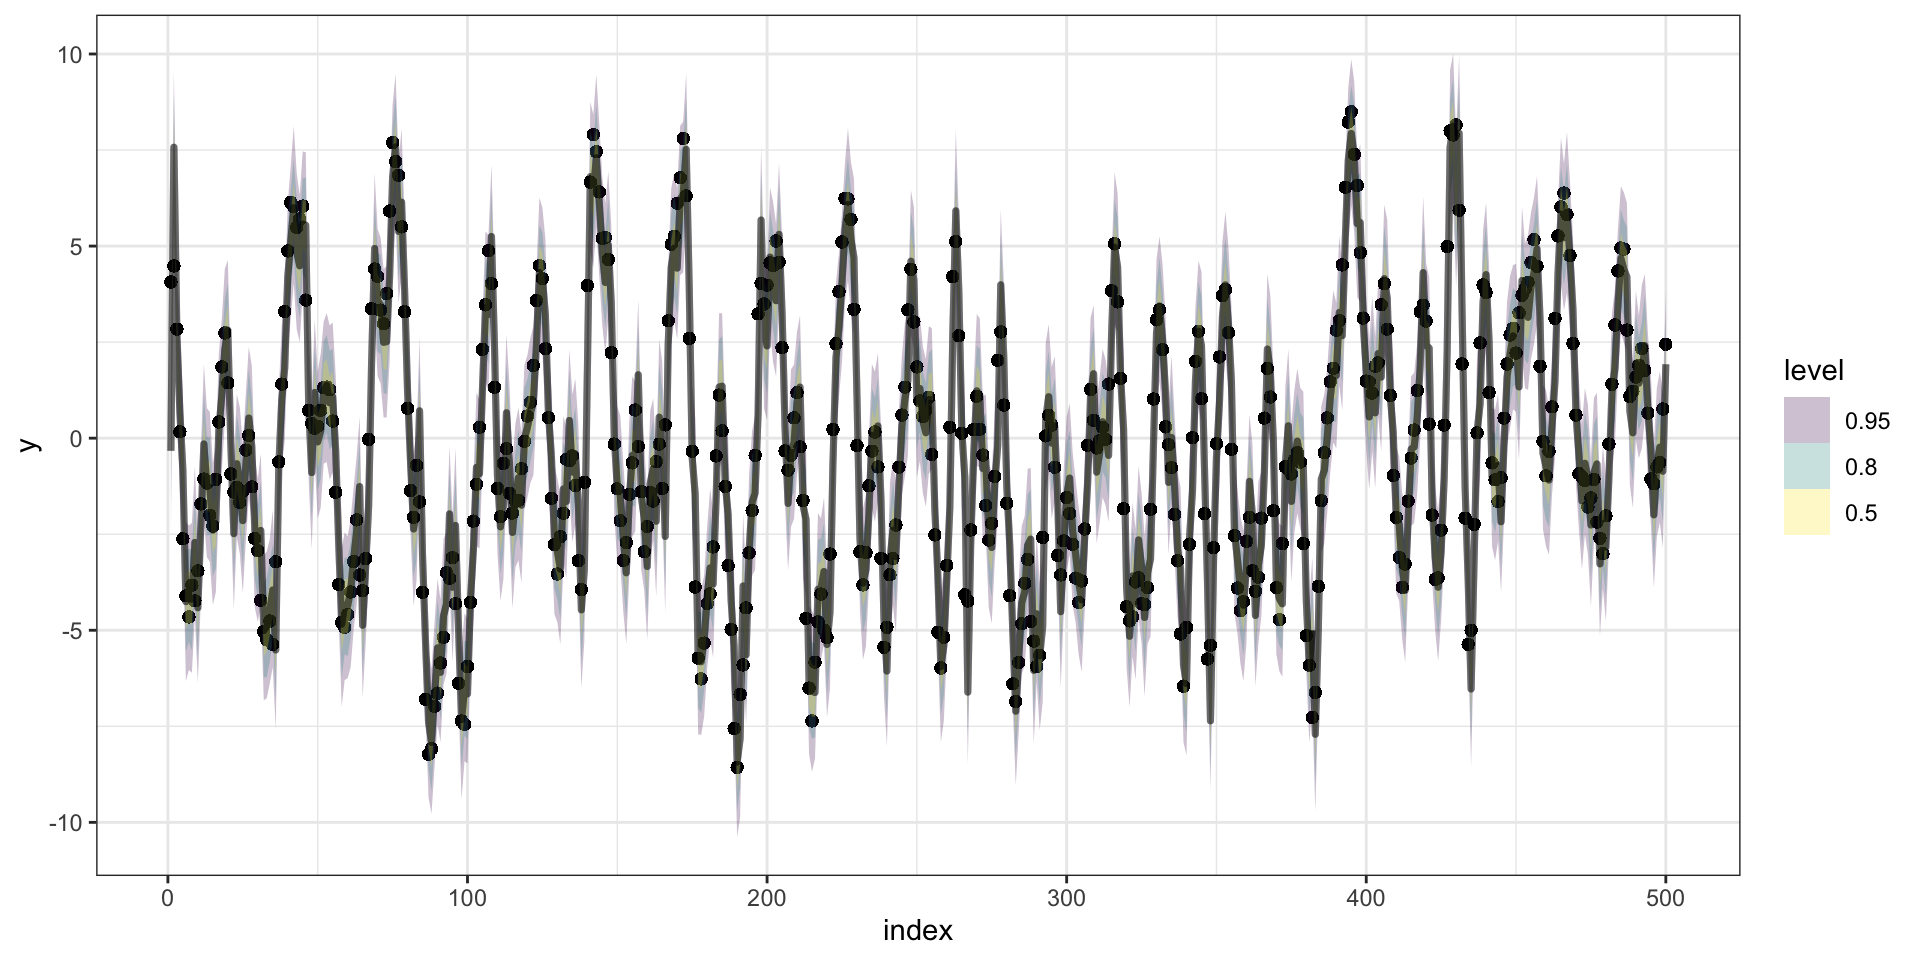
\includegraphics[width=\textwidth]{Lec13_files/figure-beamer/unnamed-chunk-32-1} \end{center}

\end{frame}

\end{document}
